\documentclass[../main.tex]{subfiles}
% ===============================================================
% Documento
% ===============================================================
\begin{document}

\begin{titlepage}
\centering

\vspace*{-3cm}

\includegraphics[height=1.5cm]{figuras/logo_fcefyn.png}
\hspace{1cm}
\includegraphics[height=2cm]{figuras/logo_ohmc.jpeg}

\vspace{5cm}

{\fontsize{33}{40}\selectfont Convenio ATLAS II \par}
\vspace{0.4cm}
{\fontsize{33}{40}\selectfont Provincia de Córdoba \par}

\vspace{0.6cm}

{\fontsize{26}{32}\selectfont \textcolor{gray}{Componente Solar} \par}

\vspace{2.5cm}

{\large
Facultad de Ciencias Exactas, Físicas y Naturales (FCEFyN) \par}

\vspace{0.15cm}

{\large
Laboratorio de Hidrometeorología \par}

\vspace{3.5cm}

{\normalsize Segundo Informe de Avance \par}
\vspace{1cm}
{\normalsize Mayo 2026 \par}

\end{titlepage}

\newpage

\section*{Resumen general}

El presente informe documenta el desarrollo y ejecución de la fase de calibración de las estaciones de superficie Davis, para el Convenio ATLAS II de la Provincia de Córdoba. Esta fase abarca la consolidación de la base de datos en superficie mediante la fusión de series históricas de la red automática Davis (2015-2019), la implementación de varios controles de calidad bajo estrictas normas, el modelado dinámico de cielo claro mediante el modelo físico de transferencia radiativa REST2 y la calibración virtual dinámica para corregir sesgos ópticos, espectrales y de coseno de los sensores de silicio. Tras procesar más de 9.04 millones de registros crudos, se obtuvo un dataset final consolidado de 3.05 millones de horas diurnas calibradas para 166 estaciones aprobadas. Finalmente, se presenta un prototipo de regionalización climática solar de la provincia mediante \textit{clustering} no supervisado. 

\bigskip

\newpage

\tableofcontents

\newpage

\section{Introducción y Estado del Convenio}

\subsection{Alcance y estado de avance del Segundo Informe}

El presente informe detalla la metodología y los resultados correspondientes a esta nueva fase del Atlas Solar Provincial. Esta etapa tiene como principal objetivo establecer una base de datos en superficie homogénea, de alta resolución temporal y con calidad controlada, destinada a la caracterización del recurso solar en la provincia de Córdoba.

La red de estaciones meteorológicas automáticas (AWS) Davis, operada de manera distribuida en el territorio por diferentes entidades gubernamentales y productivas, constituye una infraestructura invaluable para ampliar la cobertura espacial del estudio. Sin embargo, los sensores de radiación de bajo costo basados en fotodiodos de silicio que equipan estas estaciones presentan sesgos intrínsecos asociados a su respuesta espectral limitada y al error angular del difusor, conocido como error de coseno.

Para corregir estos sesgos de forma escalable, se implementó una metodología de Calibración Virtual Dinámica. A diferencia de los enfoques tradicionales, que requieren campañas de calibración física \textit{in situ} mediante comparación directa con instrumentos de referencia de alta precisión, este método construye una línea base de calibración virtual a partir de simulaciones de cielo despejado generadas con el modelo radiativo REST2 \cite{gueymard_2008_rest2}. Dichas simulaciones son impulsadas por información atmosférica proveniente de productos satelitales y de reanálisis, particularmente ERA5 \cite{hersbach_2020_era5} y CAMS \cite{inness_2019_cams}, lo que permite estimar las condiciones radiativas esperadas para cada ubicación y momento.

El carácter dinámico de la metodología radica en que la corrección aplicada no se limita a un único factor multiplicativo constante, sino que se adapta a las condiciones geométricas y operativas del sensor. En particular, el error angular asociado al difusor se modela mediante funciones polinómicas dependientes del ángulo cenital solar, permitiendo corregir la respuesta no lineal del instrumento a lo largo del día y del año. Adicionalmente, los parámetros de calibración son recalculados mediante una segmentación temporal anual, lo que permite absorber cambios en el comportamiento del sensor asociados al envejecimiento, degradación de materiales, acumulación de suciedad o intervenciones de mantenimiento.

Con el objetivo de maximizar la cobertura temporal del Atlas Solar Provincial, se completó la recuperación, integración y homogeneización de los registros históricos disponibles. La implementación de un esquema de simulación y calibración virtual adaptado al período previo a octubre de 2020 permitió extender la base de datos y consolidar series históricas de largo plazo.

Como resultado, 39 estaciones que superaron los criterios de control de calidad disponen actualmente de series temporales continuas y consistentes a lo largo de todo el período de análisis comprendido entre 2019 y 2025. Estas estaciones constituyen el núcleo de referencia temporal del Atlas Solar, proporcionando un anclaje robusto para la caracterización de la variabilidad interanual del recurso solar y para la validación de los procedimientos de regionalización y modelado espacial desarrollados en etapas posteriores del proyecto.


%\newpage

\section{Control de Calidad Físico (QC) de la Red de Superficie}

Según lo establecido en el primer informe de avance del Convenio ATLAS II - Componente Solar, la red de estaciones de superficie inicialmente seleccionada estaba conformada por 56 estaciones meteorológicas automáticas (EMAs), distribuidas de manera aproximadamente uniforme sobre el territorio provincial. Sin embargo, a partir de trabajos recientes desarrollados por el OHMC, la base de datos disponible fue ampliada significativamente, permitiendo incrementar la red de estudio a un total de 166 estaciones con series temporales de radiación solar continuas y suficientemente completas dentro del período analizado.

En consecuencia, la red actualmente utilizada queda conformada por las estaciones presentadas en la Fig. \ref{fig:mapa_red_estaciones}. Este conjunto observacional resulta considerablemente más robusto que el empleado en la versión inicial del estudio, tanto por su mayor cobertura espacial como por la mejora en la completitud temporal de las series disponibles.

\begin{figure}[H]
    \centering
    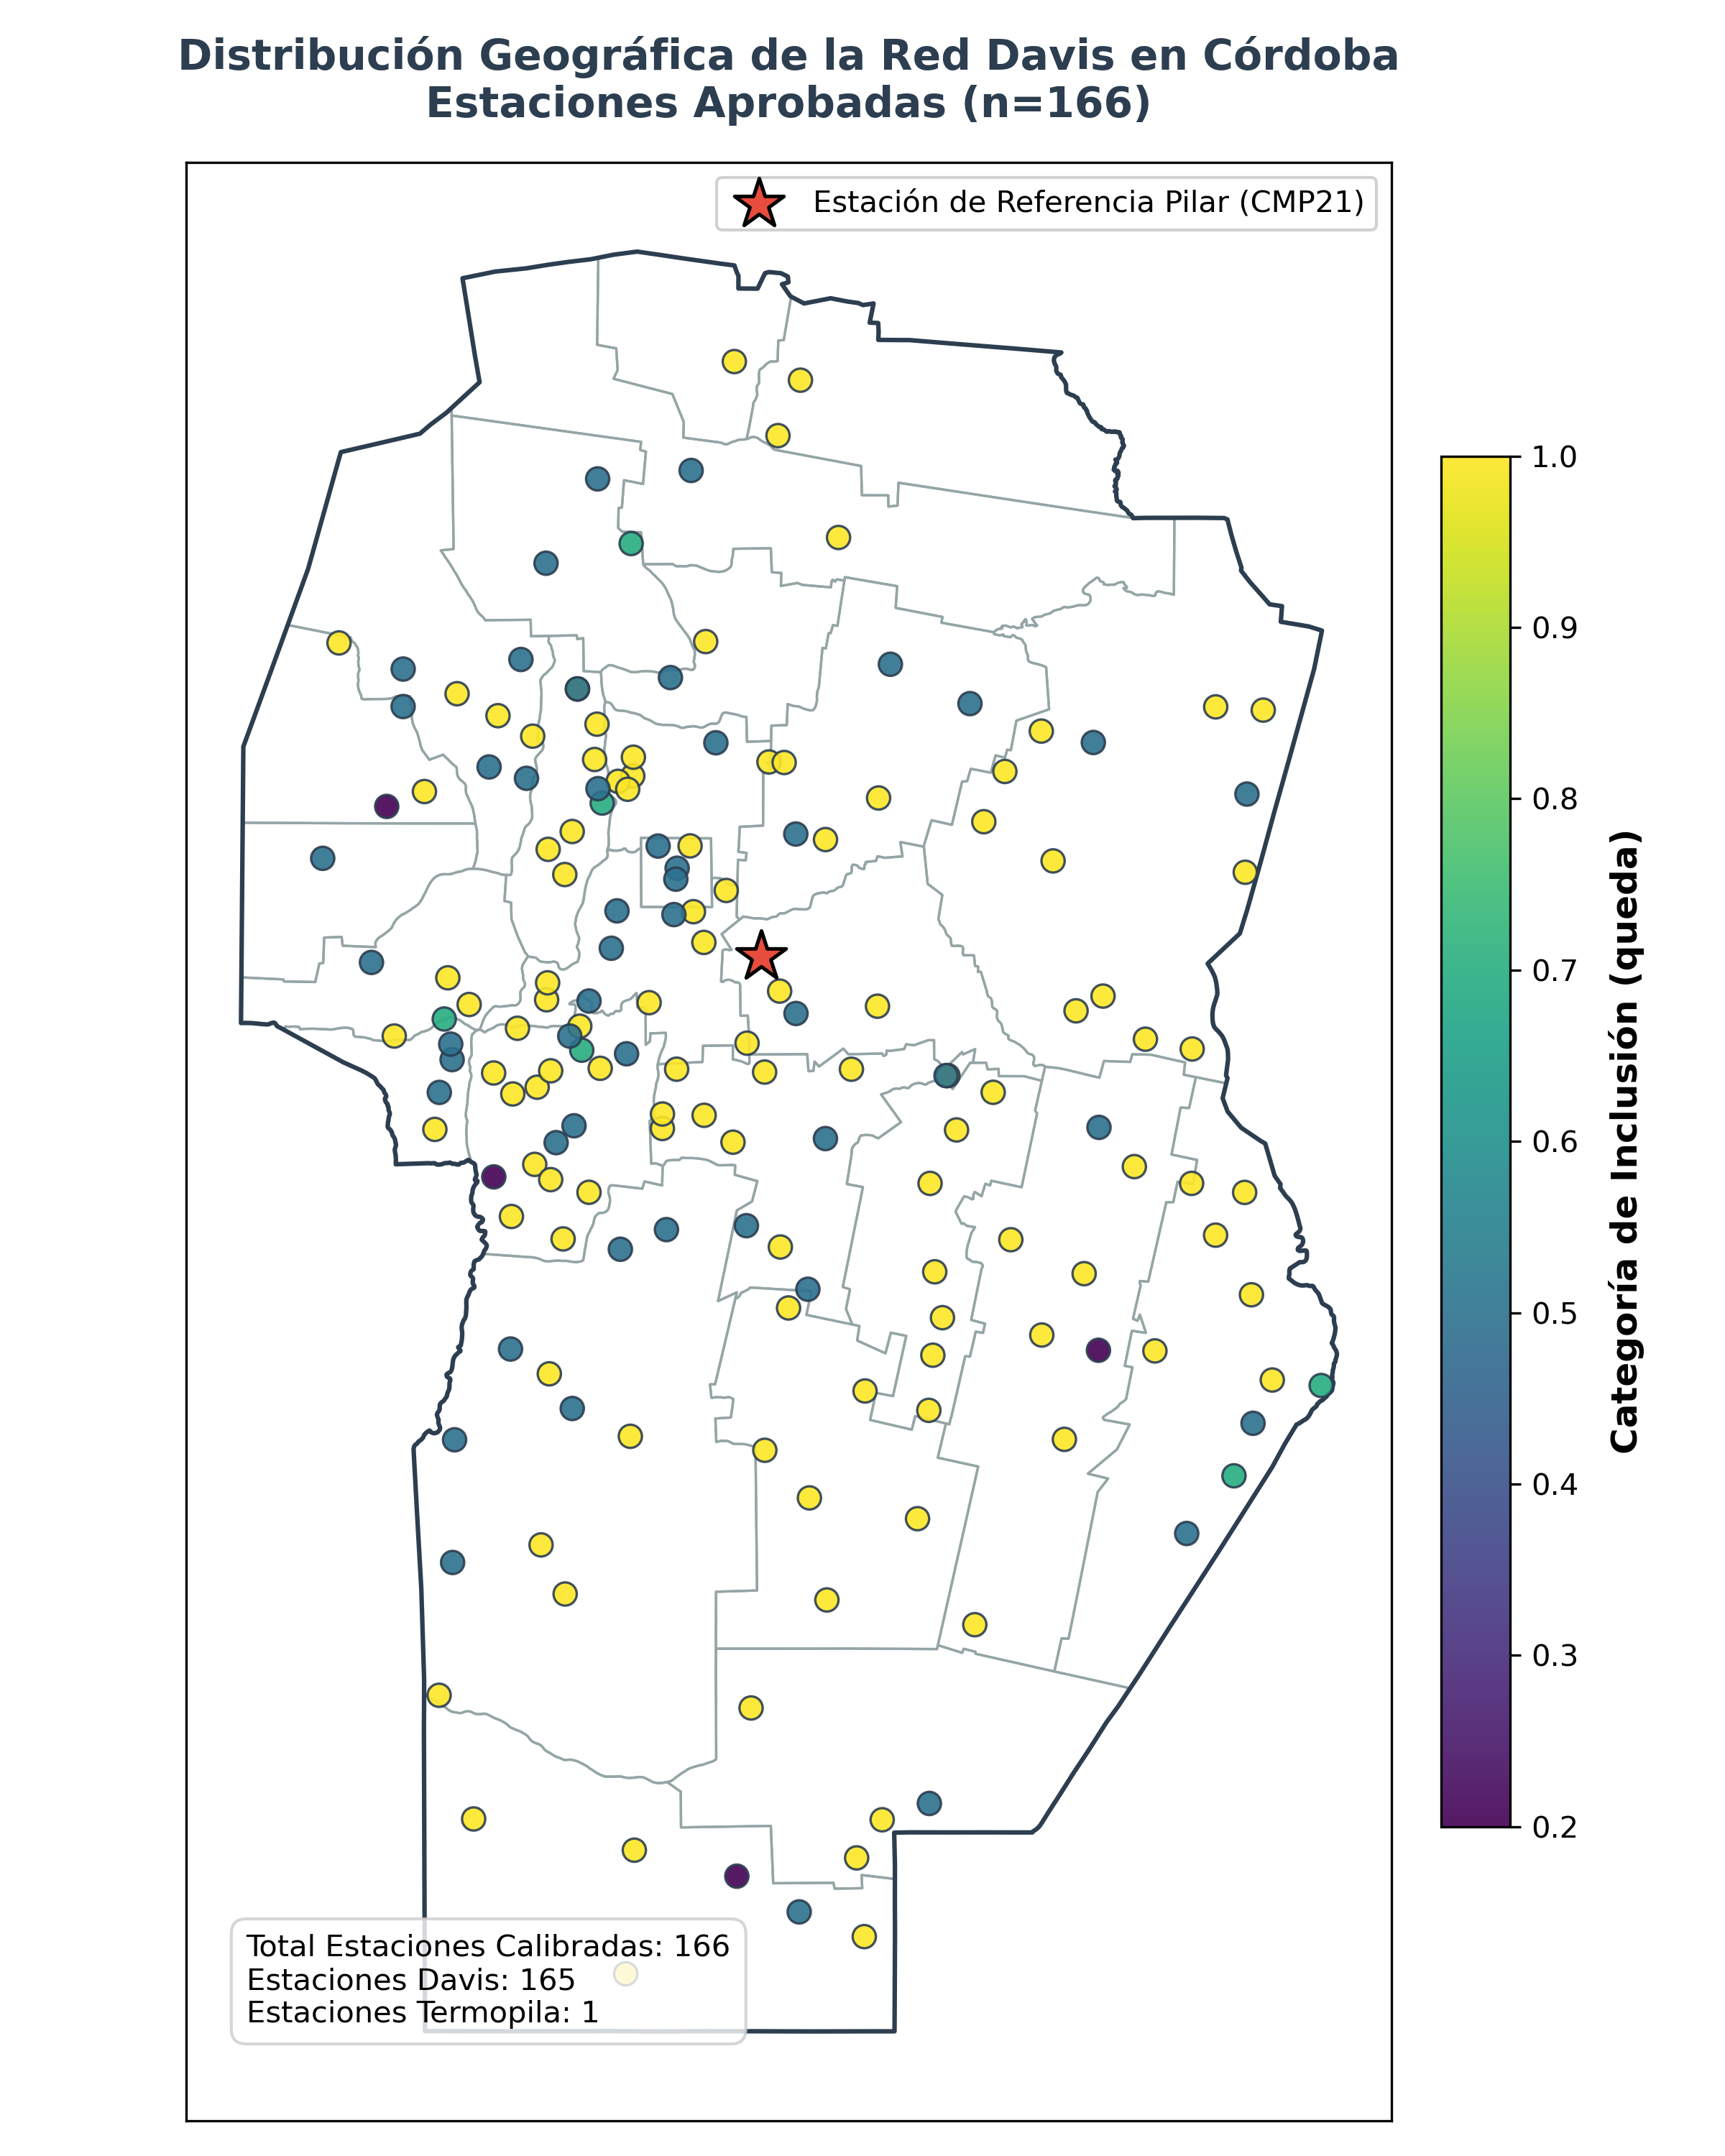
\includegraphics[width=0.75\textwidth]{figuras/figura_1_mapa_red.png}
    \caption{Mapa de EMAs seleccionadas para la calibración y futura generación del Atlas de energía solar potencial de la Provincia de Córdoba.}
    \label{fig:mapa_red_estaciones}
\end{figure}

\subsection{Protocolo de Control de Calidad de Datos Terrestres}

El procesamiento de cada serie temporal de radiación solar, correspondiente a las mediciones obtenidas en cada estación, se sometió secuencialmente al siguiente protocolo de limpieza y control de calidad, basado en criterios utilizados para el control de calidad de mediciones radiométricas de superficie \cite{long_dutton_2002,long_shi_2008}:

\begin{itemize}

    \item \textbf{Limpieza de valores no físicos:} se estableció un umbral máximo físico de 1400 W/m\textsuperscript{2} y se eliminaron todos los registros que superaron dicho valor. Asimismo, se filtraron los valores negativos de radiación solar.

    \item \textbf{Filtro de completitud anual:} se descartaron aquellas series temporales cuya completitud anual fue inferior al 70\%. Dado que se requieren series no solo continuas sino también suficientemente completas, se exigió que cada estación posea datos válidos en al menos el 70\% de las horas esperadas para cada año analizado.

    \item \textbf{Control de frecuencia intrahoraria:} se eliminaron aquellas horas con menos del 80\% de las mediciones esperadas. Este criterio busca garantizar una frecuencia de muestreo suficientemente regular dentro de cada hora. En el caso de datos con resolución temporal de 10 minutos, se requieren idealmente 6 mediciones por hora, aceptándose un mínimo de 4 registros válidos.

    \item \textbf{Agregación horaria:} debido a la elevada variabilidad de las mediciones dentro de intervalos subhorarios, se calculó la media horaria de radiación solar para cada estación, con el objetivo de reducir la influencia del ruido instrumental y de las fluctuaciones de corto plazo sobre esta variable.

\end{itemize}

\subsection{Análisis de Disponibilidad, Completitud y Homogeneidad Temporal}

En la etapa inicial de definición de la red de estaciones de superficie se priorizó tanto la distribución espacial de las EMAs como la completitud y continuidad temporal de sus series de radiación solar. En el primer informe de avance se había trabajado con una selección preliminar de 56 estaciones. Sin embargo, la ampliación posterior de la base de datos disponible permitió extender el análisis a 166 estaciones definitivas, incrementando sustancialmente la cobertura espacial y temporal del sistema observacional.

Tras aplicar el protocolo de control de calidad sobre las 166 estaciones, se evaluaron dos métricas complementarias: la tasa de retención diurna efectiva, asociada a la cantidad de datos diurnos que superan los filtros generales de calidad, y la fracción de datos seleccionados bajo condiciones de cielo claro, utilizada específicamente para el cálculo de los factores de calibración angular. Como se ilustra en la Figura \ref{fig:completitud_analisis}, la tasa media de retención diurna efectiva general fue del 87.2\%. Por su parte, la ventana estricta de cielo claro representa en promedio un 20.5\% de los datos diurnos totales, lo cual constituye una muestra suficientemente robusta para el ajuste de las curvas de calibración.

\begin{figure}[H]
    \centering
    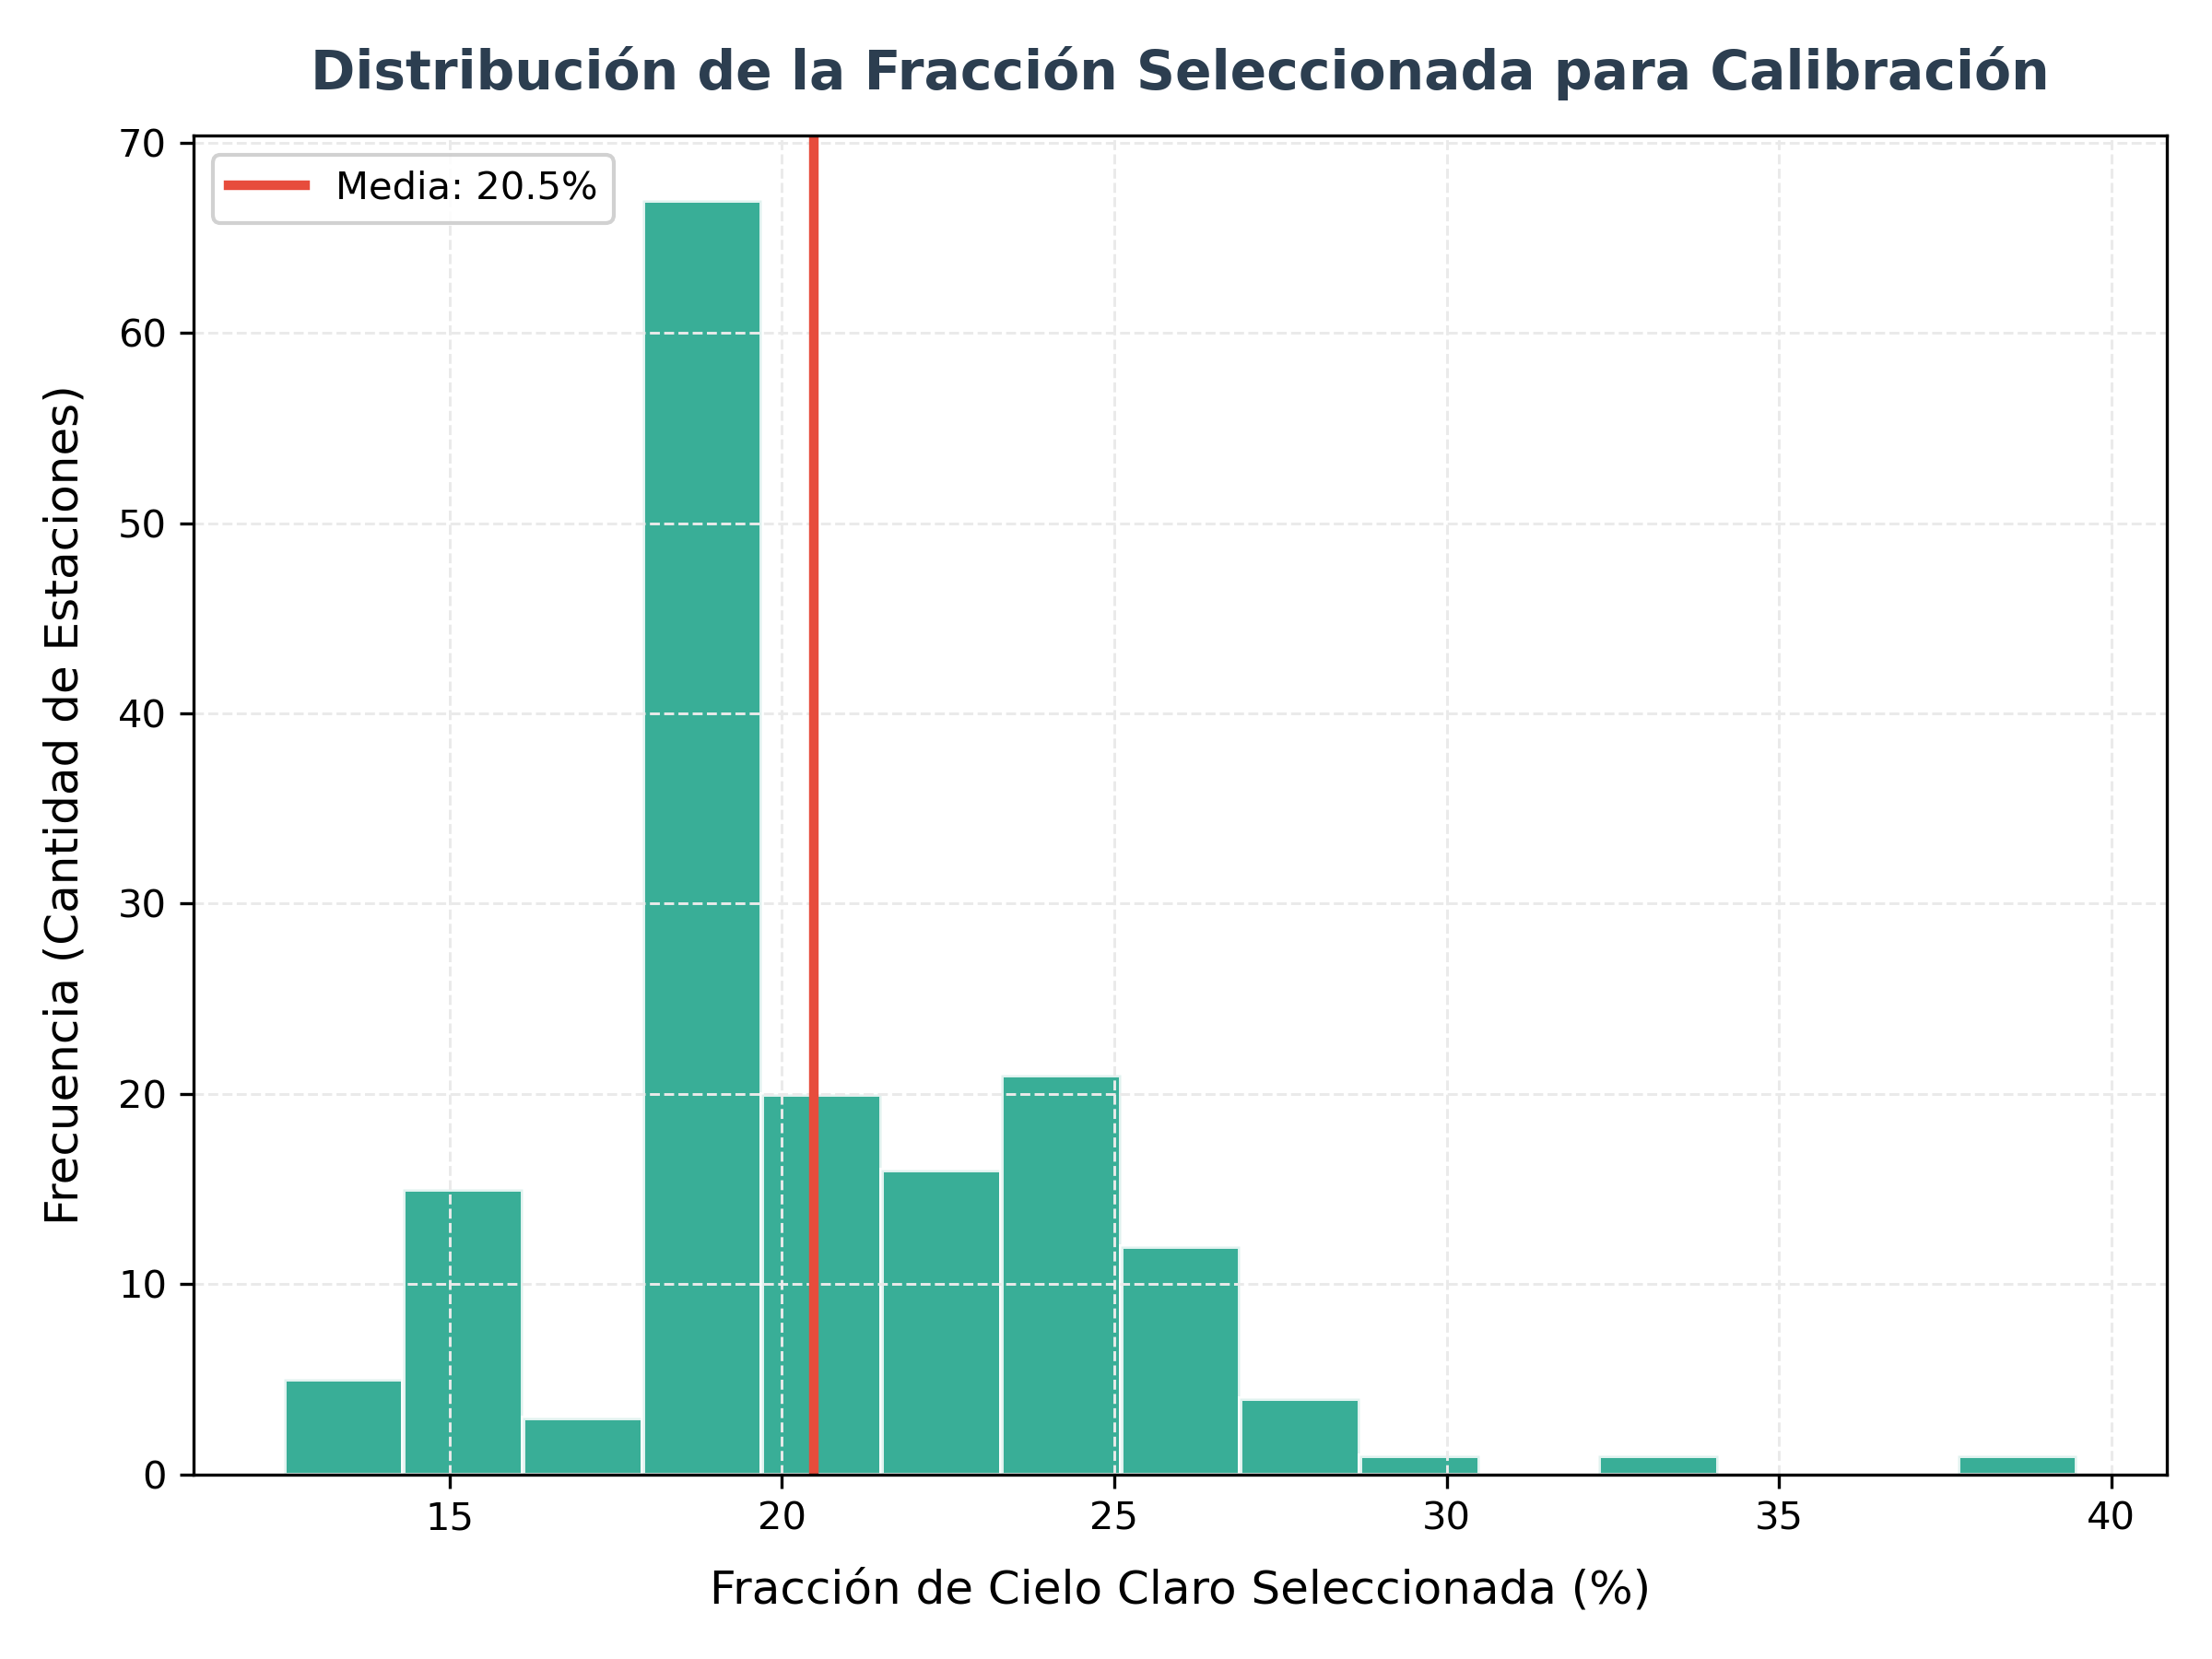
\includegraphics[width=\textwidth]{figuras/figura_5_completitud_distribucion.png}
    \caption{Distribución de la fracción de datos seleccionados para calibración bajo cielo claro.}
    \label{fig:completitud_analisis}
\end{figure}

Durante la inspección detallada de las series temporales se identificaron estaciones con cambios abruptos entre años consecutivos, reflejados en diferencias importantes en la amplitud de las mediciones y en los valores máximos observados. Estas discontinuidades sugieren posibles cambios instrumentales, modificaciones de configuración, intervenciones de mantenimiento, acumulación de suciedad, fallas parciales del sensor o desajustes en el multiplicador interno de la consola.

Dado que la red de estaciones disponible es limitada, descartar completamente estas EMAs implicaría perder una cantidad considerable de información observacional. Por este motivo, se optó por analizar cada estación de forma individual, identificando períodos temporalmente consistentes que pudieran conservarse para las etapas posteriores de calibración. Bajo esta metodología, algunas estaciones pueden incorporarse con la totalidad de sus registros, mientras que otras contribuyen únicamente con aquellos períodos que superan los controles de calidad y homogeneidad temporal.

\subsubsection{Control de Calidad Trimestral Dinámico y detección de períodos anómalos}

Como filtro final del control de calidad, se implementó un algoritmo de validación trimestral orientado a detectar períodos anómalos persistentes en las series calibradas. Este control no busca evaluar el desempeño general de la calibración, sino identificar tramos temporalmente inconsistentes que podrían responder a fallas instrumentales, cambios abruptos de configuración, obstrucción del sensor o degradación severa.

Para cada estación y trimestre, se comparó el percentil 99.9 de la serie calibrada ($P99_{cal}$) contra el percentil 99.9 del modelo REST2 ($P99_{cs}$). Si la diferencia relativa superaba un umbral de $\pm25\%$, el trimestre era rechazado. Este criterio busca minimizar el rechazo de anomalías climáticas legítimas, como humo o polvo, y actuar principalmente como un filtro de inconsistencias instrumentales persistentes. Mediante este procedimiento se identificaron y eliminaron selectivamente 63 trimestres anómalos, equivalentes al 1.9\% de los trimestres evaluados.

La Figura \ref{fig:qc_trimestral} muestra dos ejemplos representativos del efecto del filtro trimestral. En el primer caso se observa una falla por sobreestimación, con picos irreales durante 2020--2021. En el segundo caso se identifica una falla por subestimación persistente durante 2025, compatible con un sensor obstruido, degradado o parcialmente fuera de servicio. En ambos casos, el filtro permite enmascarar los períodos anómalos sin descartar la totalidad de la estación.

\begin{figure}[H]
    \centering
    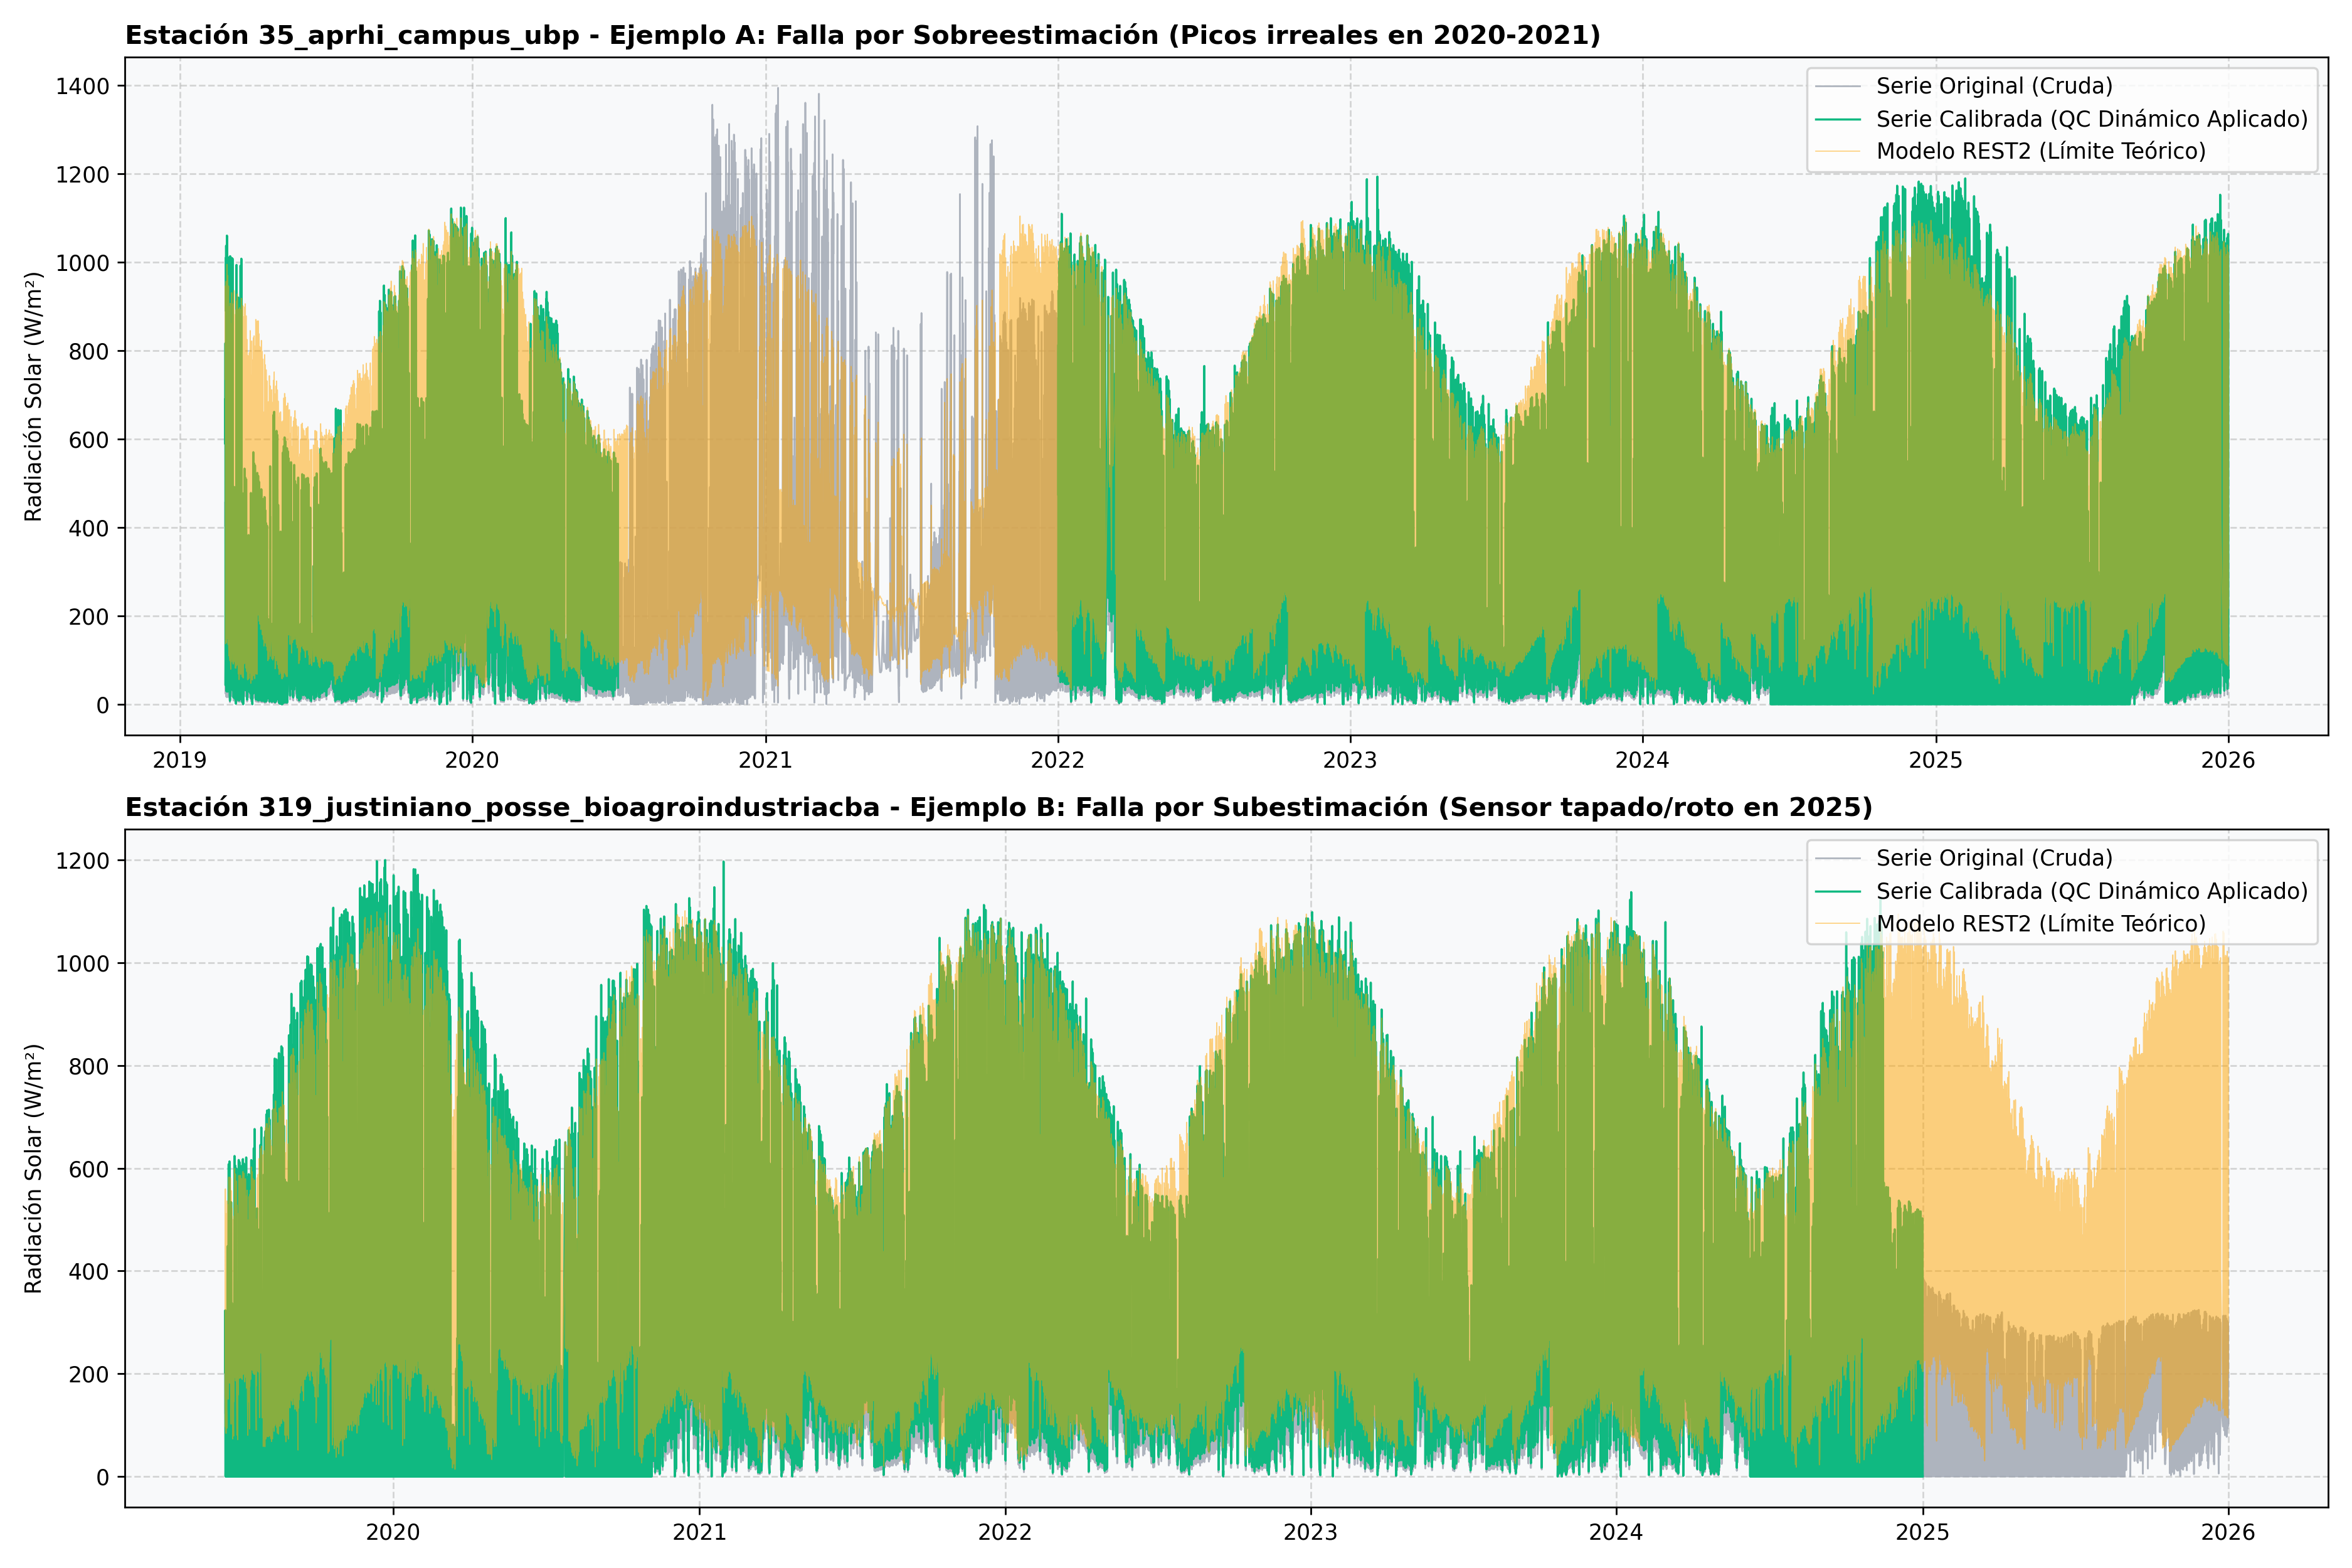
\includegraphics[width=0.95\textwidth]{figuras/figura_qc_trimestral_efecto.png}
    \caption{Ejemplos del efecto del Control de Calidad Trimestral Dinámico. Las brechas visualizan períodos anómalos persistentes que fueron identificados y enmascarados como NaN, evitando el descarte completo de estaciones con tramos parcialmente utilizables.}
    \label{fig:qc_trimestral}
\end{figure}



\section{Simulación de Cielo Claro REST2: el Calibrador Virtual}

\subsection{Configuración y parametrización del modelo REST2}

Para evitar depender de una grilla satelital intermedia, que podría introducir sesgos espaciales adicionales, se proyectó el estado atmosférico sobre la coordenada exacta de cada estación mediante interpolación trilineal en tiempo, latitud y longitud. Para ello se utilizaron variables provenientes de ERA5 \cite{hersbach_2020_era5} y CAMS \cite{inness_2019_cams}, incorporadas al modelo REST2 junto con la geometría solar correspondiente a cada instante de cálculo \cite{reda_andreas_2004,holmgren_2018_pvlib}.

Las principales variables atmosféricas utilizadas fueron:

\begin{itemize} 
\item \textbf{Espesor Óptico de Aerosoles (AOD):} obtenido de la base de datos CAMS (\textit{Copernicus Atmosphere Monitoring Service}) a 550 nm \cite{inness_2019_cams}. 
\item \textbf{Agua Precipitable Total (PWV):} obtenida del reanálisis global ERA5 \cite{hersbach_2020_era5}. \item \textbf{Presión Atmosférica en Superficie ($P_s$):} obtenida de ERA5 y corregida localmente por la altitud de cada estación \cite{hersbach_2020_era5}. \end{itemize}

\subsection{Generación de la base de cielo claro de referencia}

Con los parámetros atmosféricos interpolados y la geometría solar calculada para cada estación, se ejecutó el modelo físico de cielo claro REST2 \cite{gueymard_2008_rest2}. Este modelo proporciona la irradiancia global horizontal teórica bajo condiciones de cielo despejado ($GHI_{cs}$) para cada hora útil en las 166 estaciones analizadas.

La serie sintética de $GHI_{cs}$ constituye la referencia fundamental, o \textit{Calibrador Virtual}, contra la cual se contrasta la señal empírica registrada por los fotodiodos de silicio. A partir de esta comparación se derivan los factores de corrección necesarios para compensar los sesgos espectrales, angulares y de escala presentes en los sensores Davis.


\section{Calibración de sensores de silicio (Red Davis) mediante REST2} 

\subsection{Metodología de calibración virtual relativa} 

Para cada estación, se seleccionaron los datos correspondientes a cielos despejados mediante un filtro de estabilidad temporal sobre la serie observada:

\begin{equation}
    \sigma_{3h}\left(\frac{GHI_{\text{obs}}}{GHI_{cs}}\right) \leq 0.03
\end{equation}

Donde $\sigma_{3h}$ es la desviación estándar móvil de 3 horas. El umbral empírico del 3\% fue seleccionado tras pruebas de sensibilidad para aislar rigurosamente ventanas libres de nubes, reteniendo una cantidad significativa de datos ($N>100$) para el ajuste.

La calibración se realizó de manera segmentada por año, permitiendo adaptar los coeficientes de corrección a cambios graduales o abruptos en el comportamiento de cada sensor. Esta decisión metodológica permite absorber variaciones asociadas al envejecimiento del instrumento, degradación de materiales, acumulación de suciedad, intervenciones de mantenimiento o cambios de configuración.

\subsection{Modelado de la respuesta angular y espectral}

La principal limitación física del fotodiodo de silicio empleado por las estaciones Davis es su respuesta espectral incompleta. Como se ilustra conceptualmente en la Fig. \ref{fig:espectro_silicio}, este tipo de sensor presenta sensibilidad principalmente en un rango aproximado de 400 nm a 1100 nm, por lo que su respuesta se reduce significativamente fuera de esa ventana, especialmente en parte del infrarrojo. Dado que la proporción espectral de la radiación solar varía con el ángulo cenital y con el camino óptico atmosférico, esta limitación introduce un sesgo espectral dependiente de la geometría solar.

\begin{figure}[H]
    \centering
    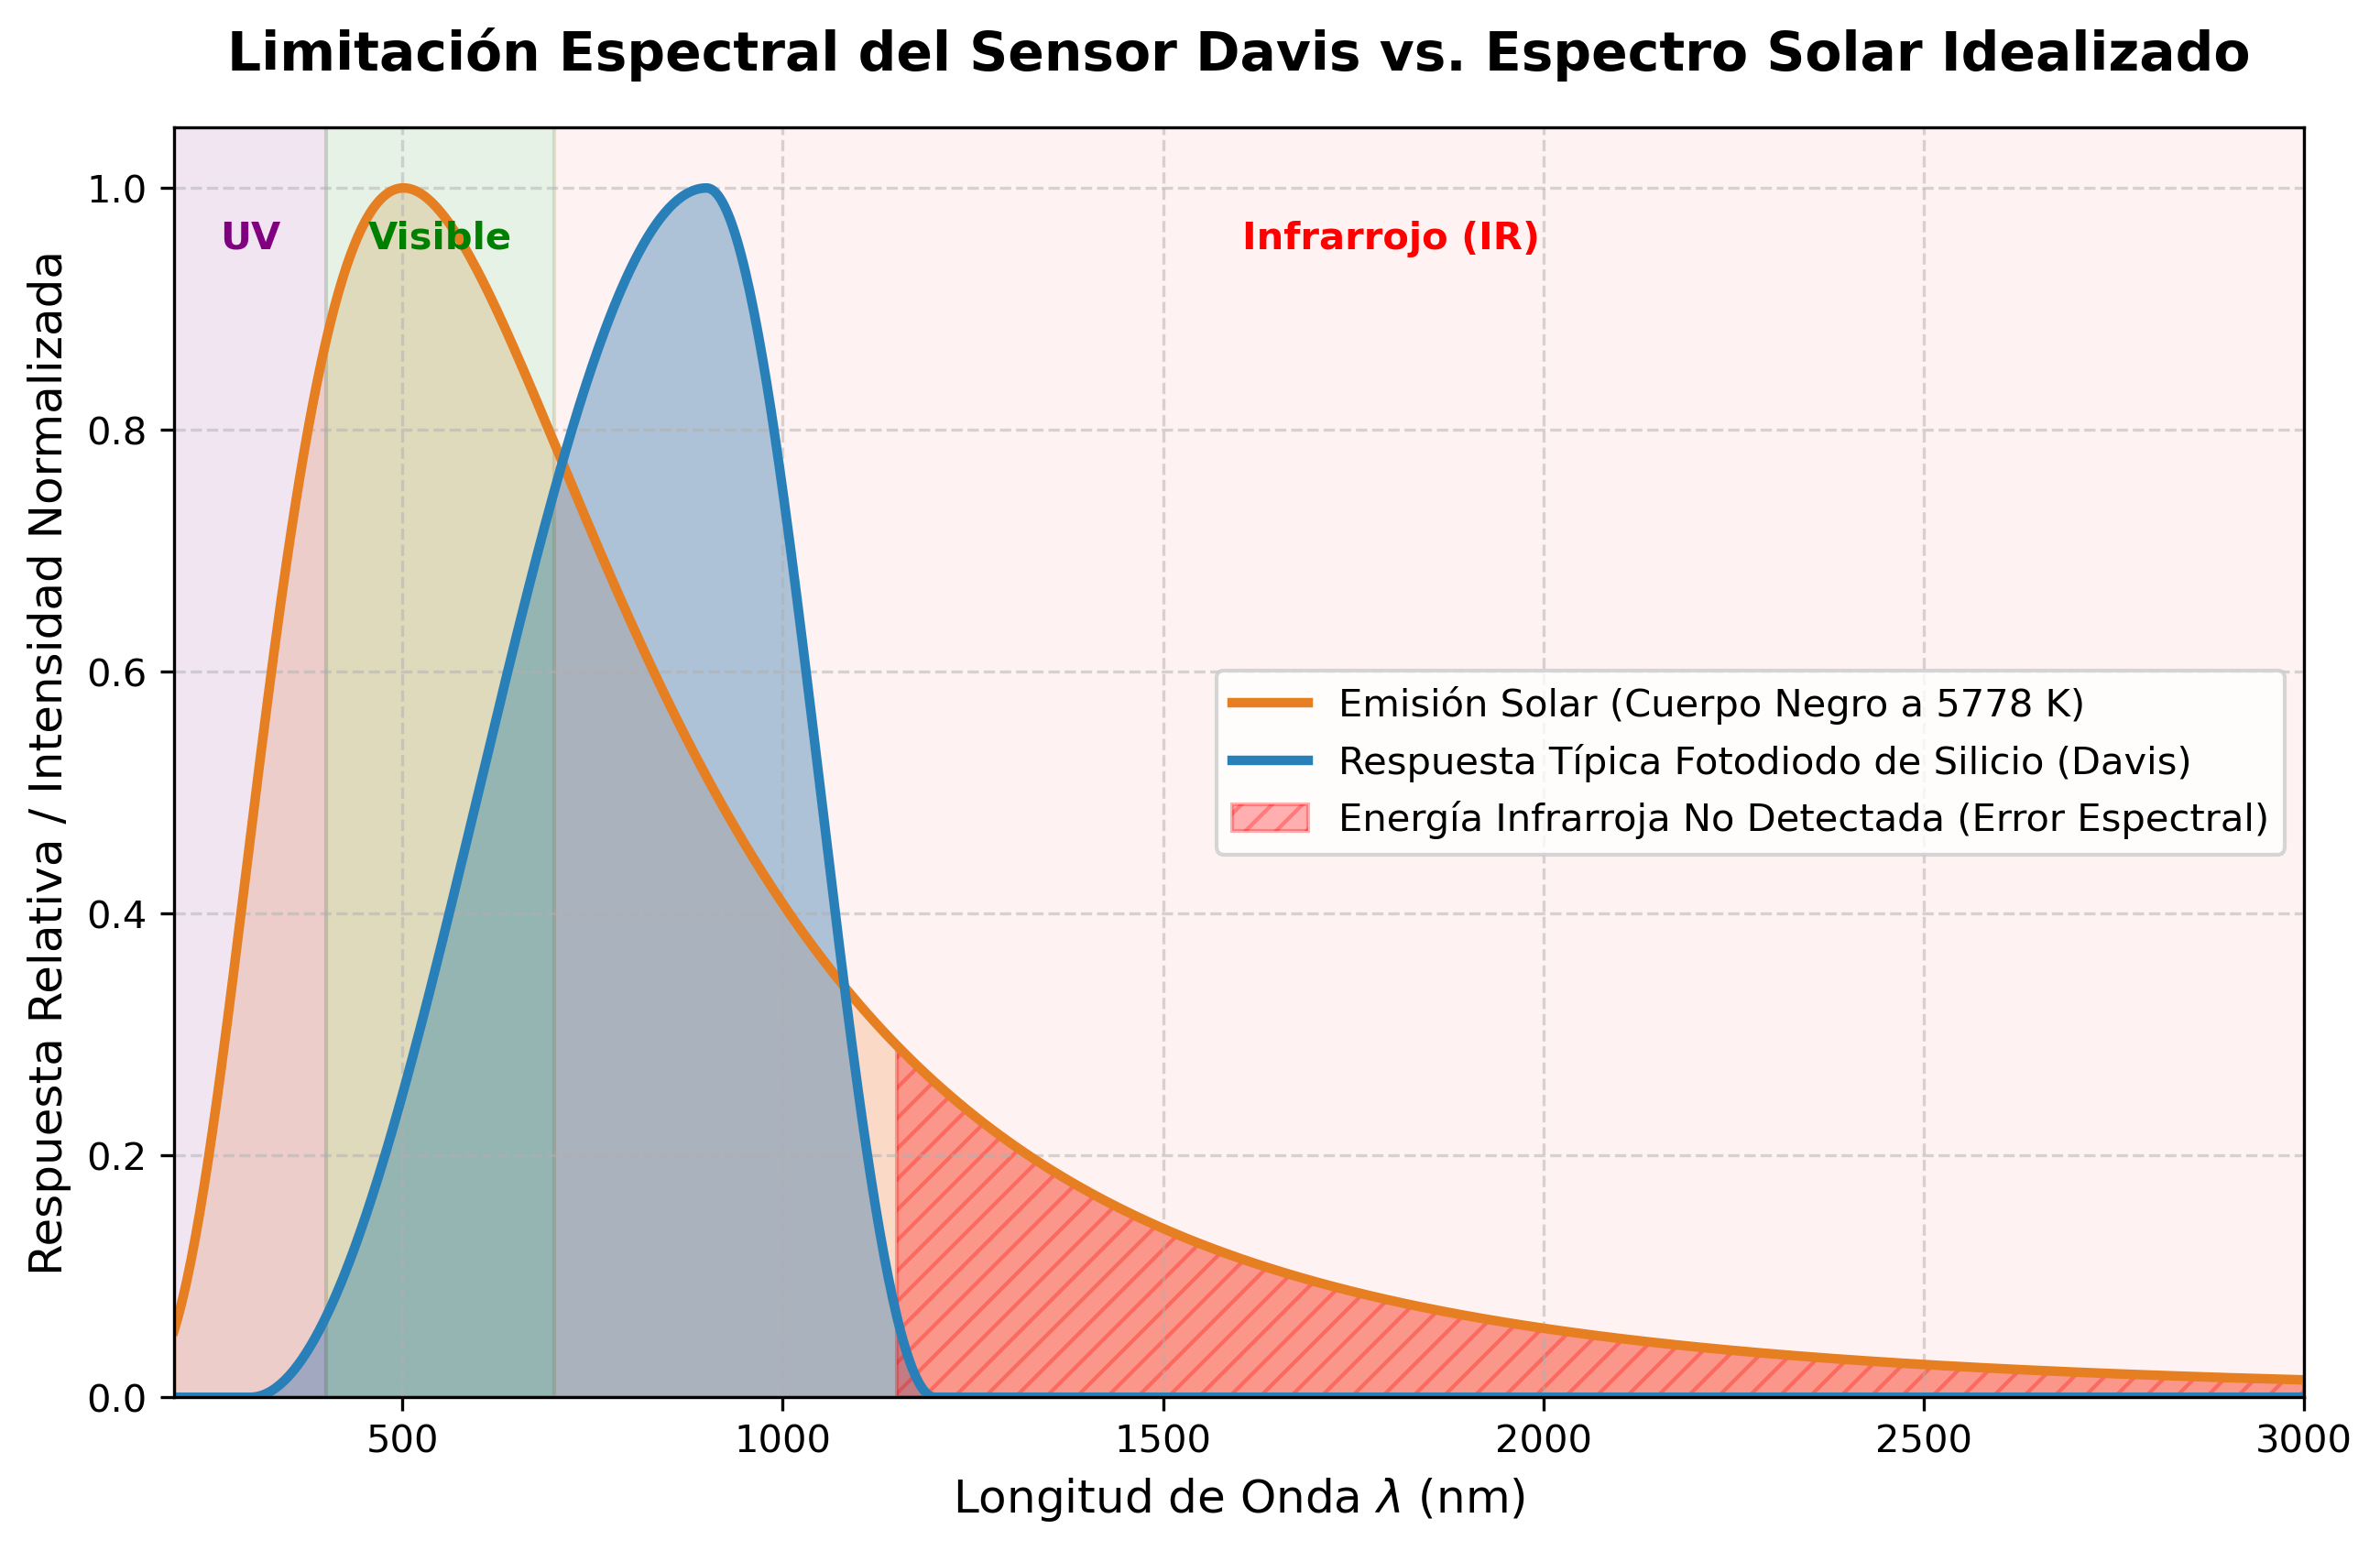
\includegraphics[width=0.85\textwidth]{figuras/figura_espectro_silicio.png}
    \caption{Representación conceptual de la limitación espectral de un fotodiodo de silicio frente a la emisión solar idealizada como cuerpo negro a 5778 K. La curva azul muestra la respuesta típica de un fotodiodo de silicio, mientras que el área sombreada indica la porción infrarroja de la irradiancia solar que no es detectada eficientemente por el sensor.}
    \label{fig:espectro_silicio}
\end{figure}

A este efecto se suma el error angular de coseno provocado por el difusor acrílico del sensor. Para corregir ambos sesgos, se propuso un factor multiplicativo dinámico dependiente de la posición solar: 

\begin{equation} 
K(\cos\theta_z) = \frac{GHI_{cs}}{GHI_{\text{obs}}} \end{equation} 

Siguiendo trabajos previos sobre dependencia angular y comparación de instrumentos radiométricos \cite{vignola_2017_photodiode}, este factor se modeló mediante un ajuste polinomial cuadrático, suficiente para capturar la respuesta no lineal del sensor sin introducir sobreajuste:

\begin{equation}
    K(\cos\theta_z) = c_0 + c_1 \cos\theta_z + c_2 \cos^2\theta_z
\end{equation}

\subsection{Resultados de la Calibración de Estaciones}

Las curvas de calibración obtenidas reflejan de manera consistente los sesgos físicos esperados en los sensores Davis. En promedio, la red presenta una subestimación de la radiación a mediodía, asociada principalmente a la respuesta espectral limitada del fotodiodo de silicio. A menores alturas solares, el factor de corrección aumenta debido al error angular del difusor, que reduce la respuesta efectiva del sensor bajo incidencia oblicua.

En términos medios, el sensor original subestima la radiación real en aproximadamente un 6.0\% bajo condiciones de sol alto ($\cos\theta_z \approx 1$). Para condiciones de sol bajo ($\cos\theta_z \approx 0.5$), el factor $K$ alcanza un valor promedio de aproximadamente 1.14, equivalente a una subestimación del orden del 14.0\%.

\begin{figure}[H]
    \centering
    \begin{subfigure}[b]{0.65\textwidth}
        \centering
        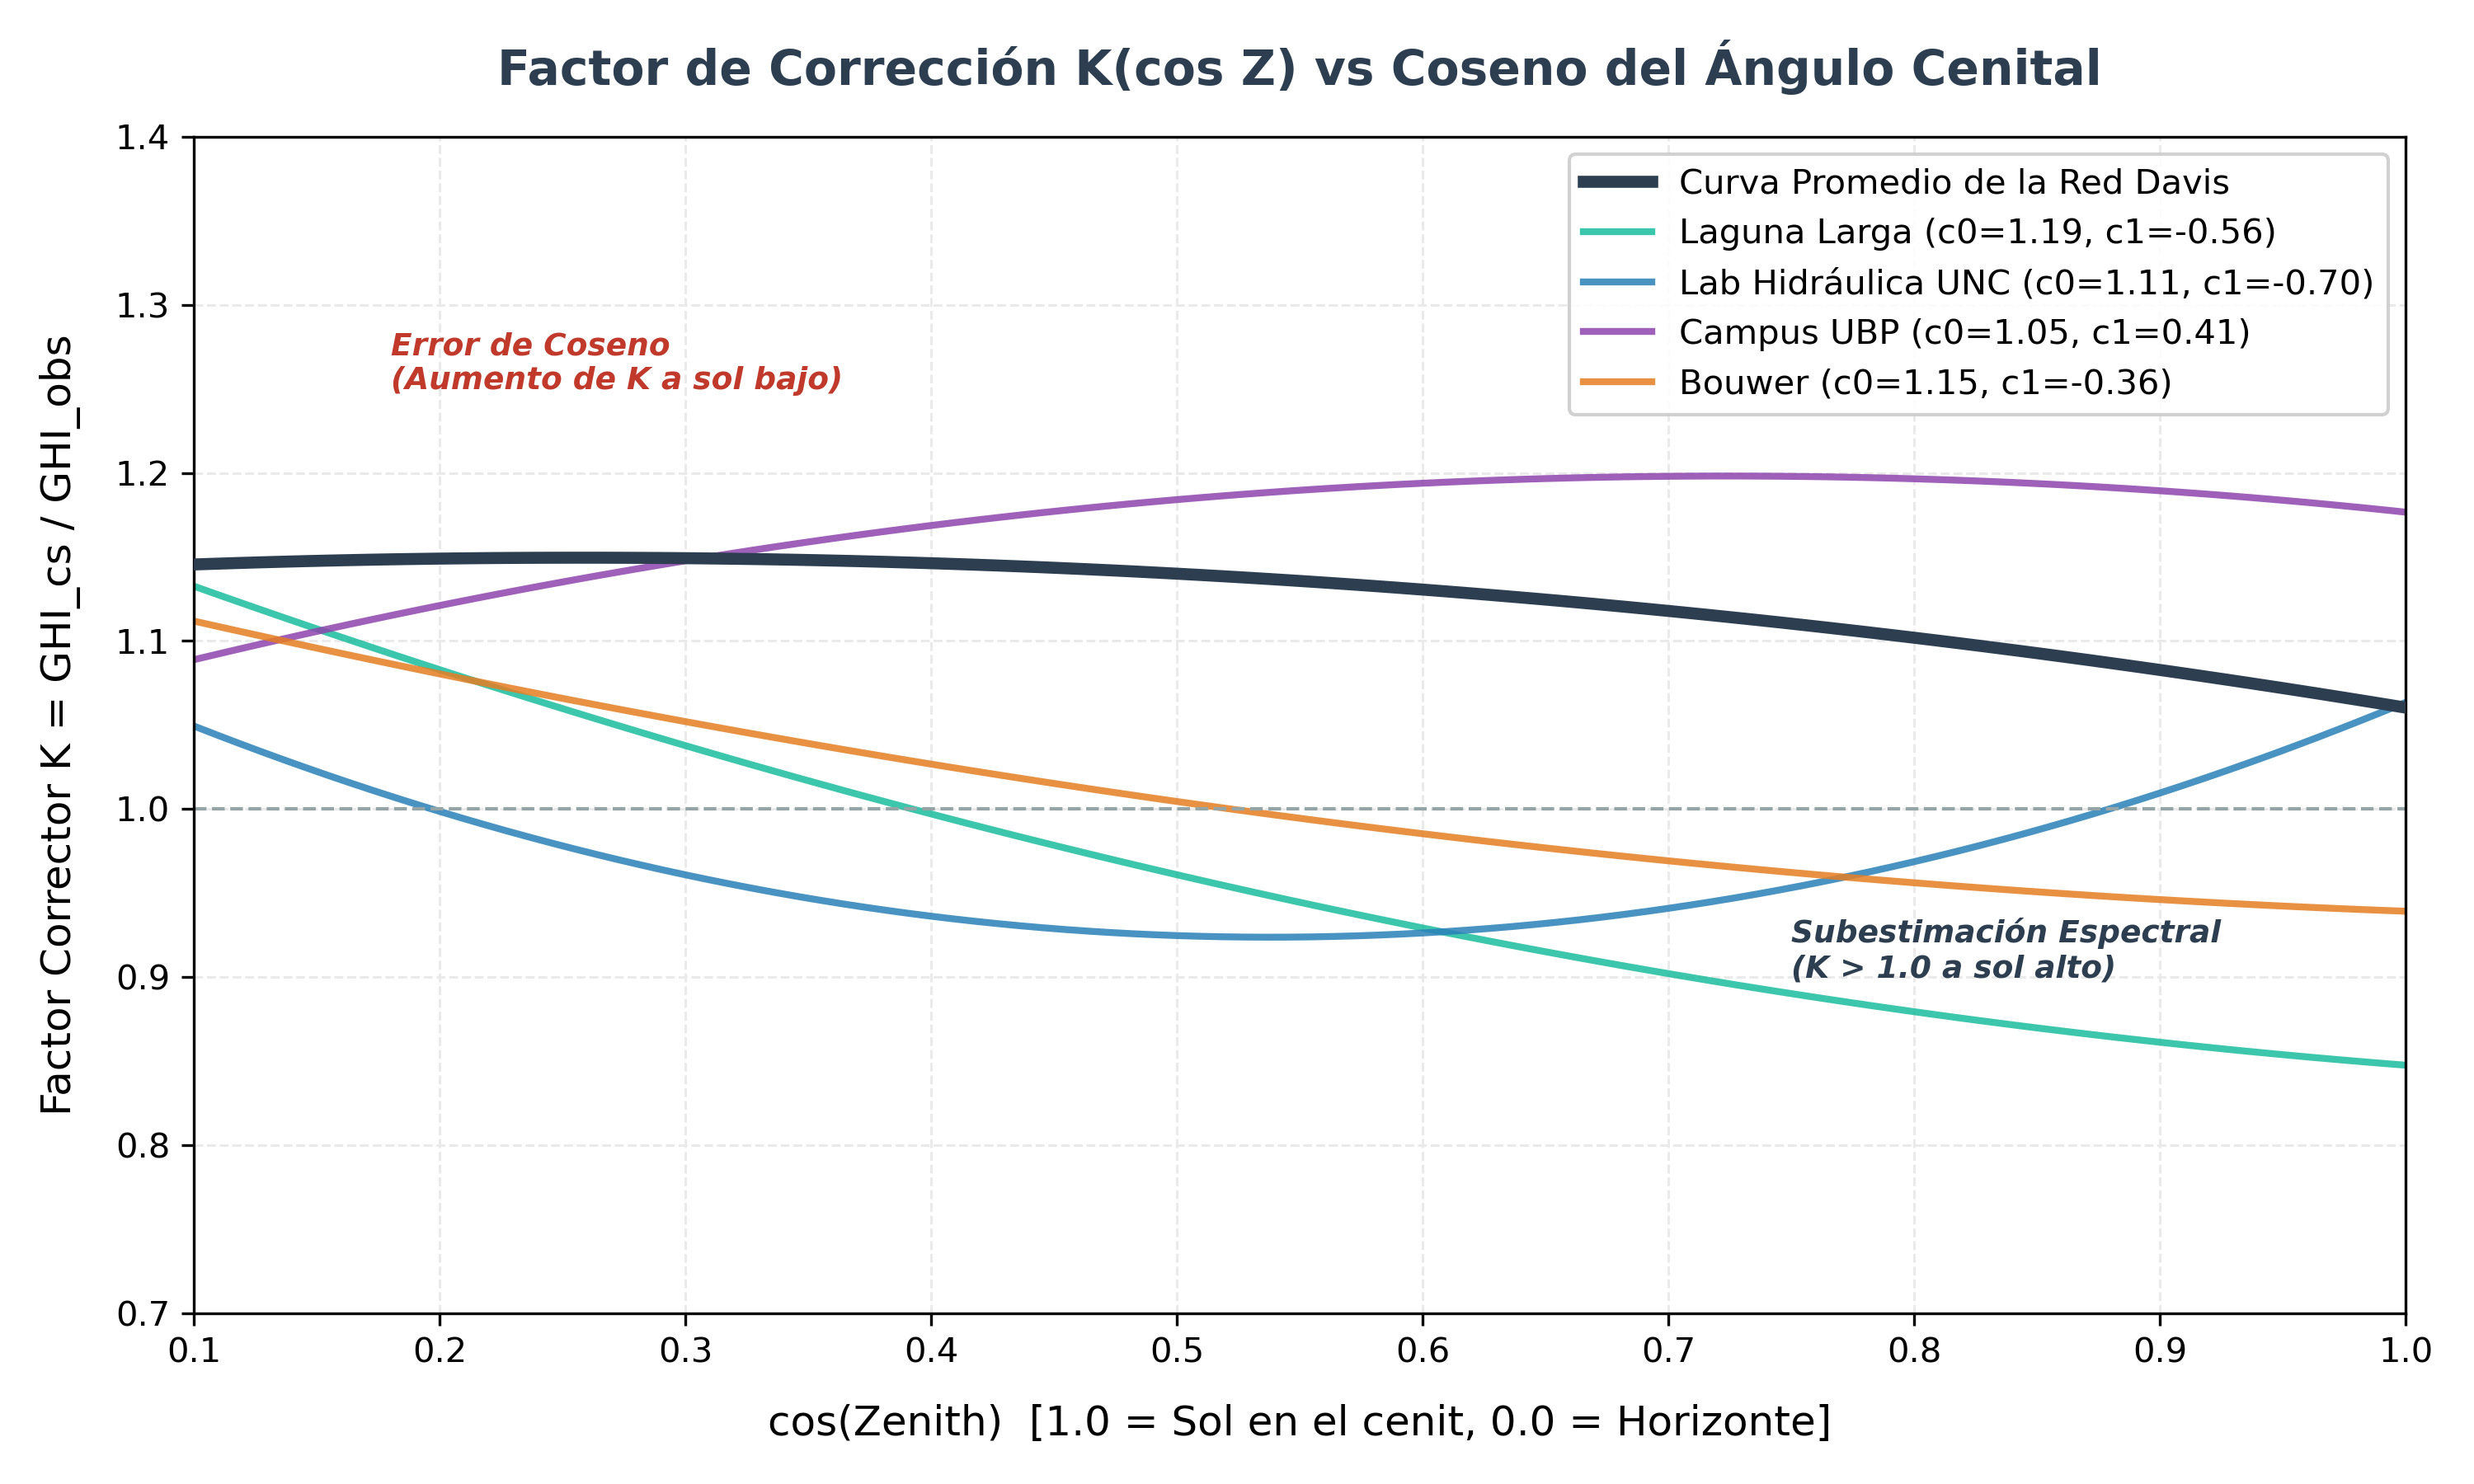
\includegraphics[width=\textwidth]{figuras/figura_2_curvas_calibracion.png}
        \caption{Curvas de calibración $K(\cos\theta_z)$.}
    \end{subfigure}
    \hfill
    \begin{subfigure}[b]{0.65\textwidth}
        \centering
        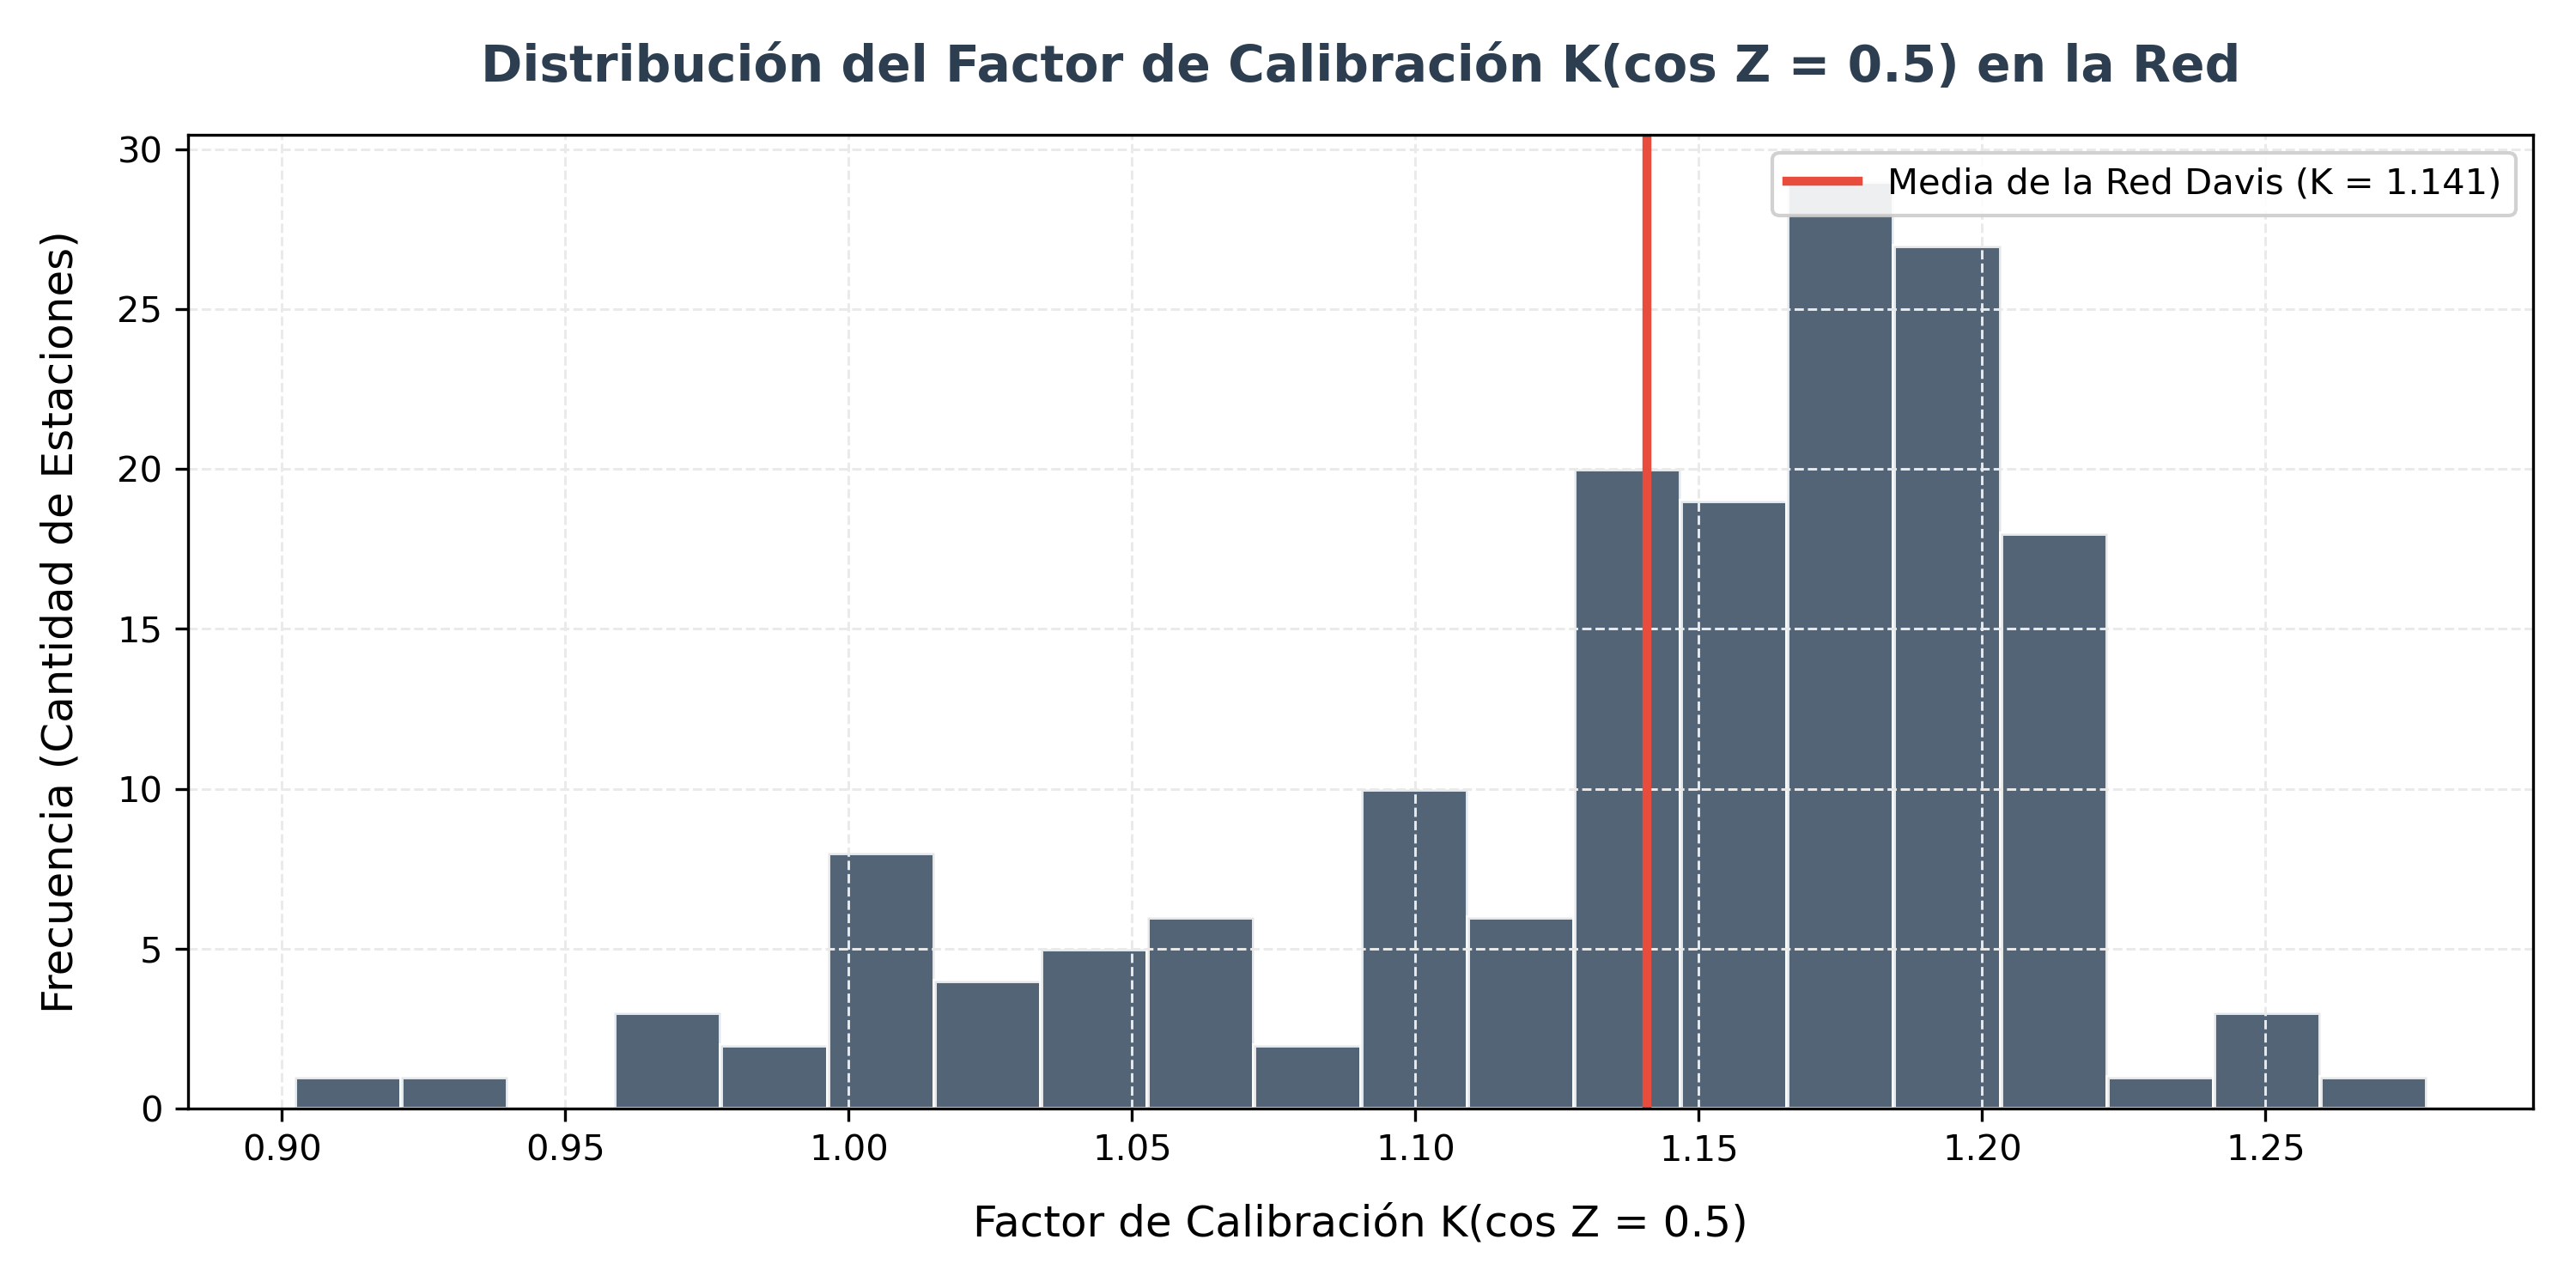
\includegraphics[width=\textwidth]{figuras/figura_4_histograma_factores.png}
        \caption{Histograma de $K$ para $\cos\theta_z = 0.5$.}
    \end{subfigure}
    \caption{Resultados del modelo de calibración angular aplicado a la red Davis.}
    \label{fig:curvas_calibracion}
\end{figure}

La estación Villa Valeria constituye un caso representativo de estaciones con saltos estructurales o cambios de régimen instrumental. Esta estación presenta discontinuidades evidentes en distintos períodos de la serie, incluyendo episodios de fuerte sobreestimación del orden de $\sim 20\%$, compatibles con posibles desajustes en el multiplicador interno de la consola.

La calibración segmentada por año permitió separar la información en tramos homogéneos, absorber cambios estructurales en la respuesta del sensor e invertir la curva de corrección cuando fue necesario. De esta manera, fue posible recuperar parte de los datos que inicialmente hubieran sido descartados, extendiendo la cobertura temporal útil sin relajar los criterios de control de calidad establecidos.

\begin{figure}[H]
    \centering
    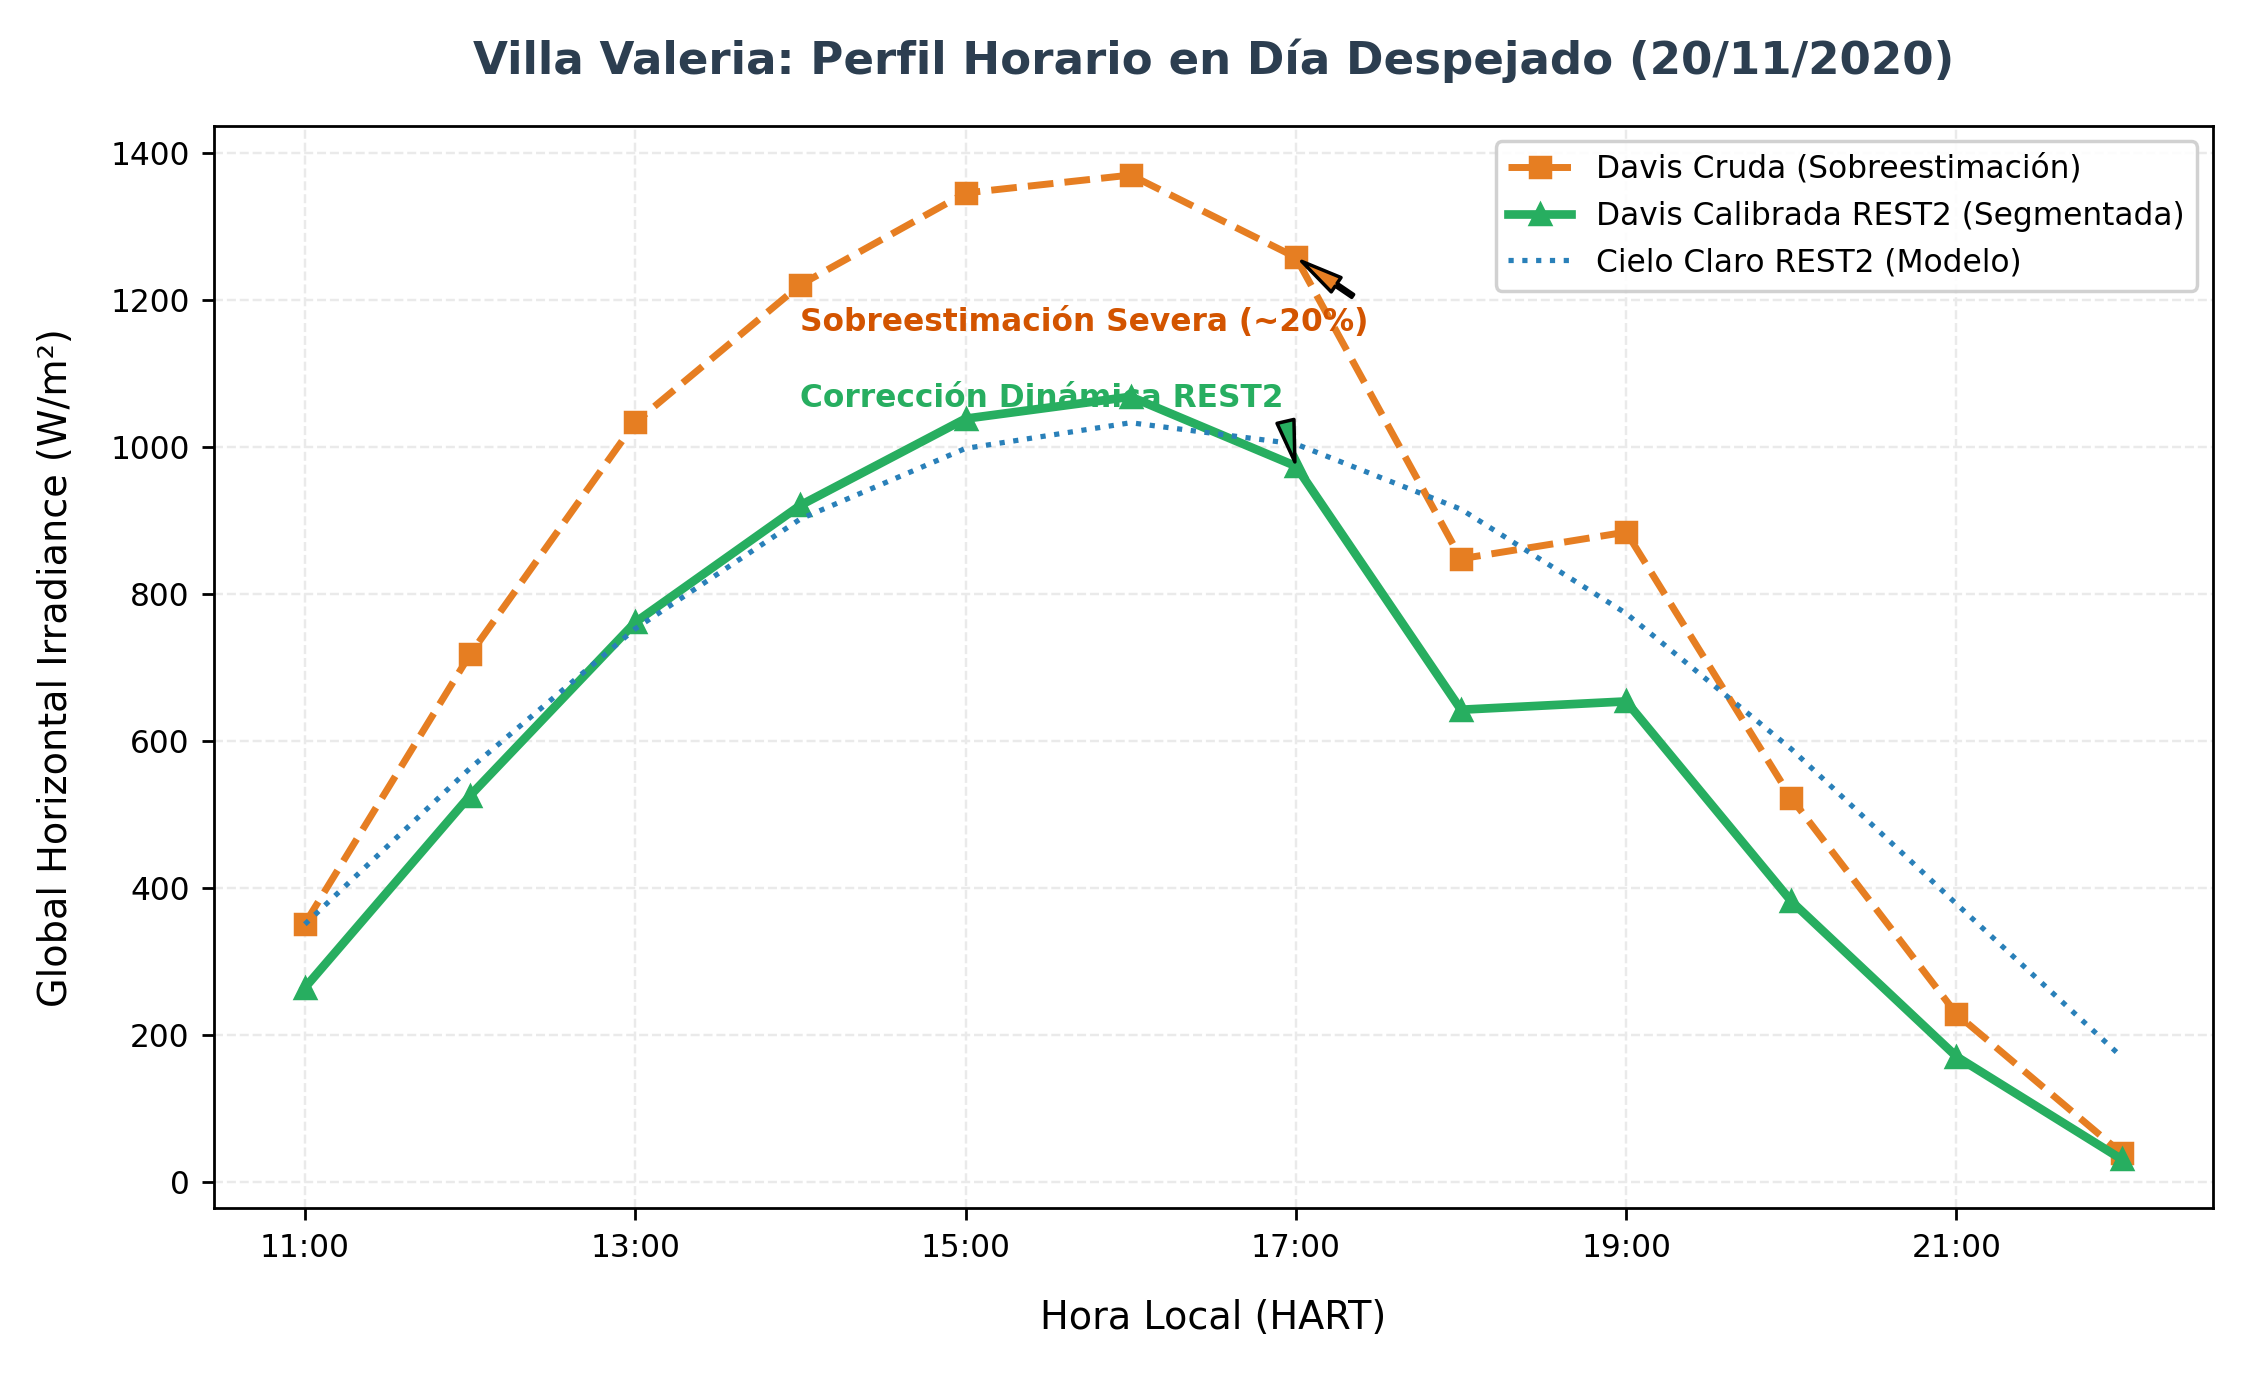
\includegraphics[width=0.75\textwidth]{figuras/figura_12_comparacion_villa_valeria.png}
    \caption{Perfil horario en Villa Valeria bajo condiciones de cielo despejado. Se observa la sobreestimación severa de la señal cruda y su corrección dinámica hacia el límite físico estimado por REST2.}
    \label{fig:villa_valeria_dia}
\end{figure}

\begin{figure}[H]
    \centering
    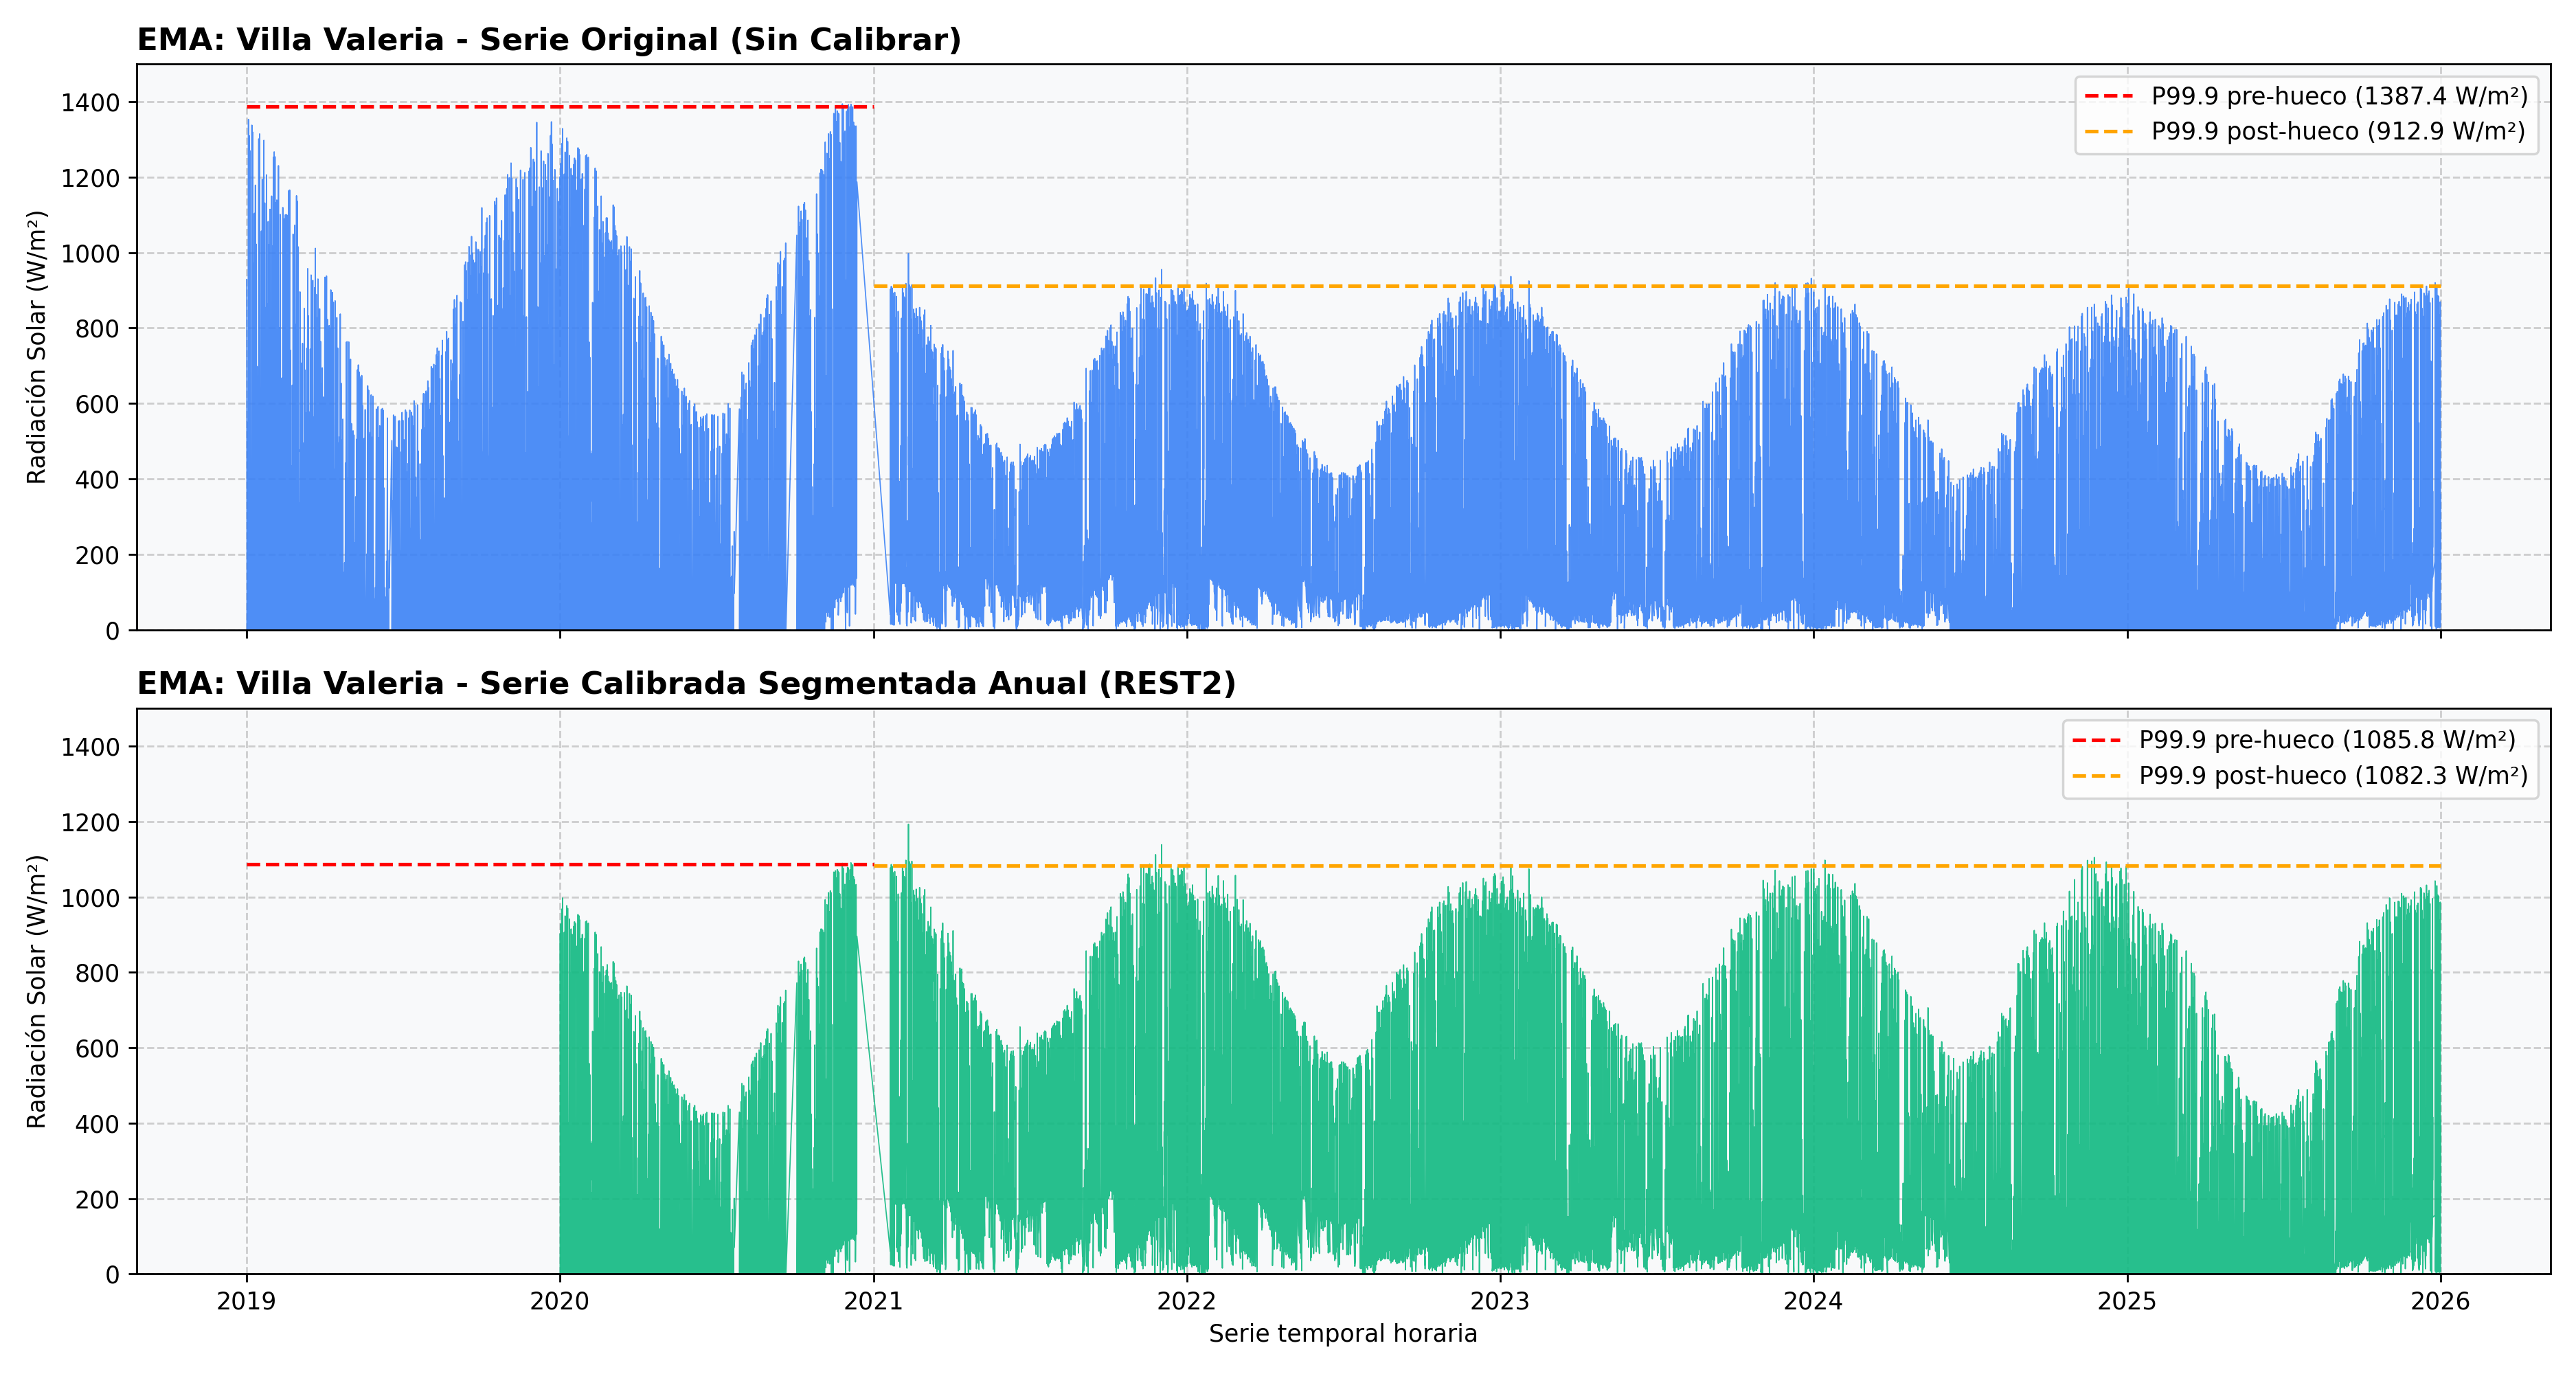
\includegraphics[width=0.95\textwidth]{figuras/figura_villa_valeria_antes_despues.png}
    \caption{Comparativa de la serie temporal de Villa Valeria antes y después de la calibración segmentada anual. Los niveles máximos se estabilizan tras la corrección, permitiendo recuperar períodos parcialmente afectados por discontinuidades instrumentales.}
    \label{fig:villa_valeria_serie}
\end{figure}

\newpage

\section{Validación de la calibración de superficie}

\subsection{Validación cruzada bajo cielo claro}

La validación empírica se realizó comparando la estación Davis Laguna Larga con el piranómetro de termopila CMP21 de Pilar, utilizado como referencia radiométrica independiente. Ambas estaciones se encuentran separadas por aproximadamente 12.3 km, en una zona de llanura con baja variabilidad topográfica relativa, lo que permite una comparación razonable bajo condiciones atmosféricas suficientemente homogéneas.

Es importante señalar que Laguna Larga constituye un caso particular dentro de la red. Mientras que la red Davis, en promedio, tiende a subestimar la radiación solar y por lo tanto requiere factores de corrección $K > 1$, esta estación presentaba una sobreestimación marcada de la irradiancia, del orden de $+20\%$. Este comportamiento es compatible con un posible desajuste local del multiplicador interno de la consola o con una configuración instrumental no homogénea respecto del resto de la red. En este caso, el procedimiento de calibración generó un factor atenuador efectivo ($K < 1$), corrigiendo la señal cruda hacia valores más consistentes con la referencia física.

\begin{figure}[H]
    \centering
    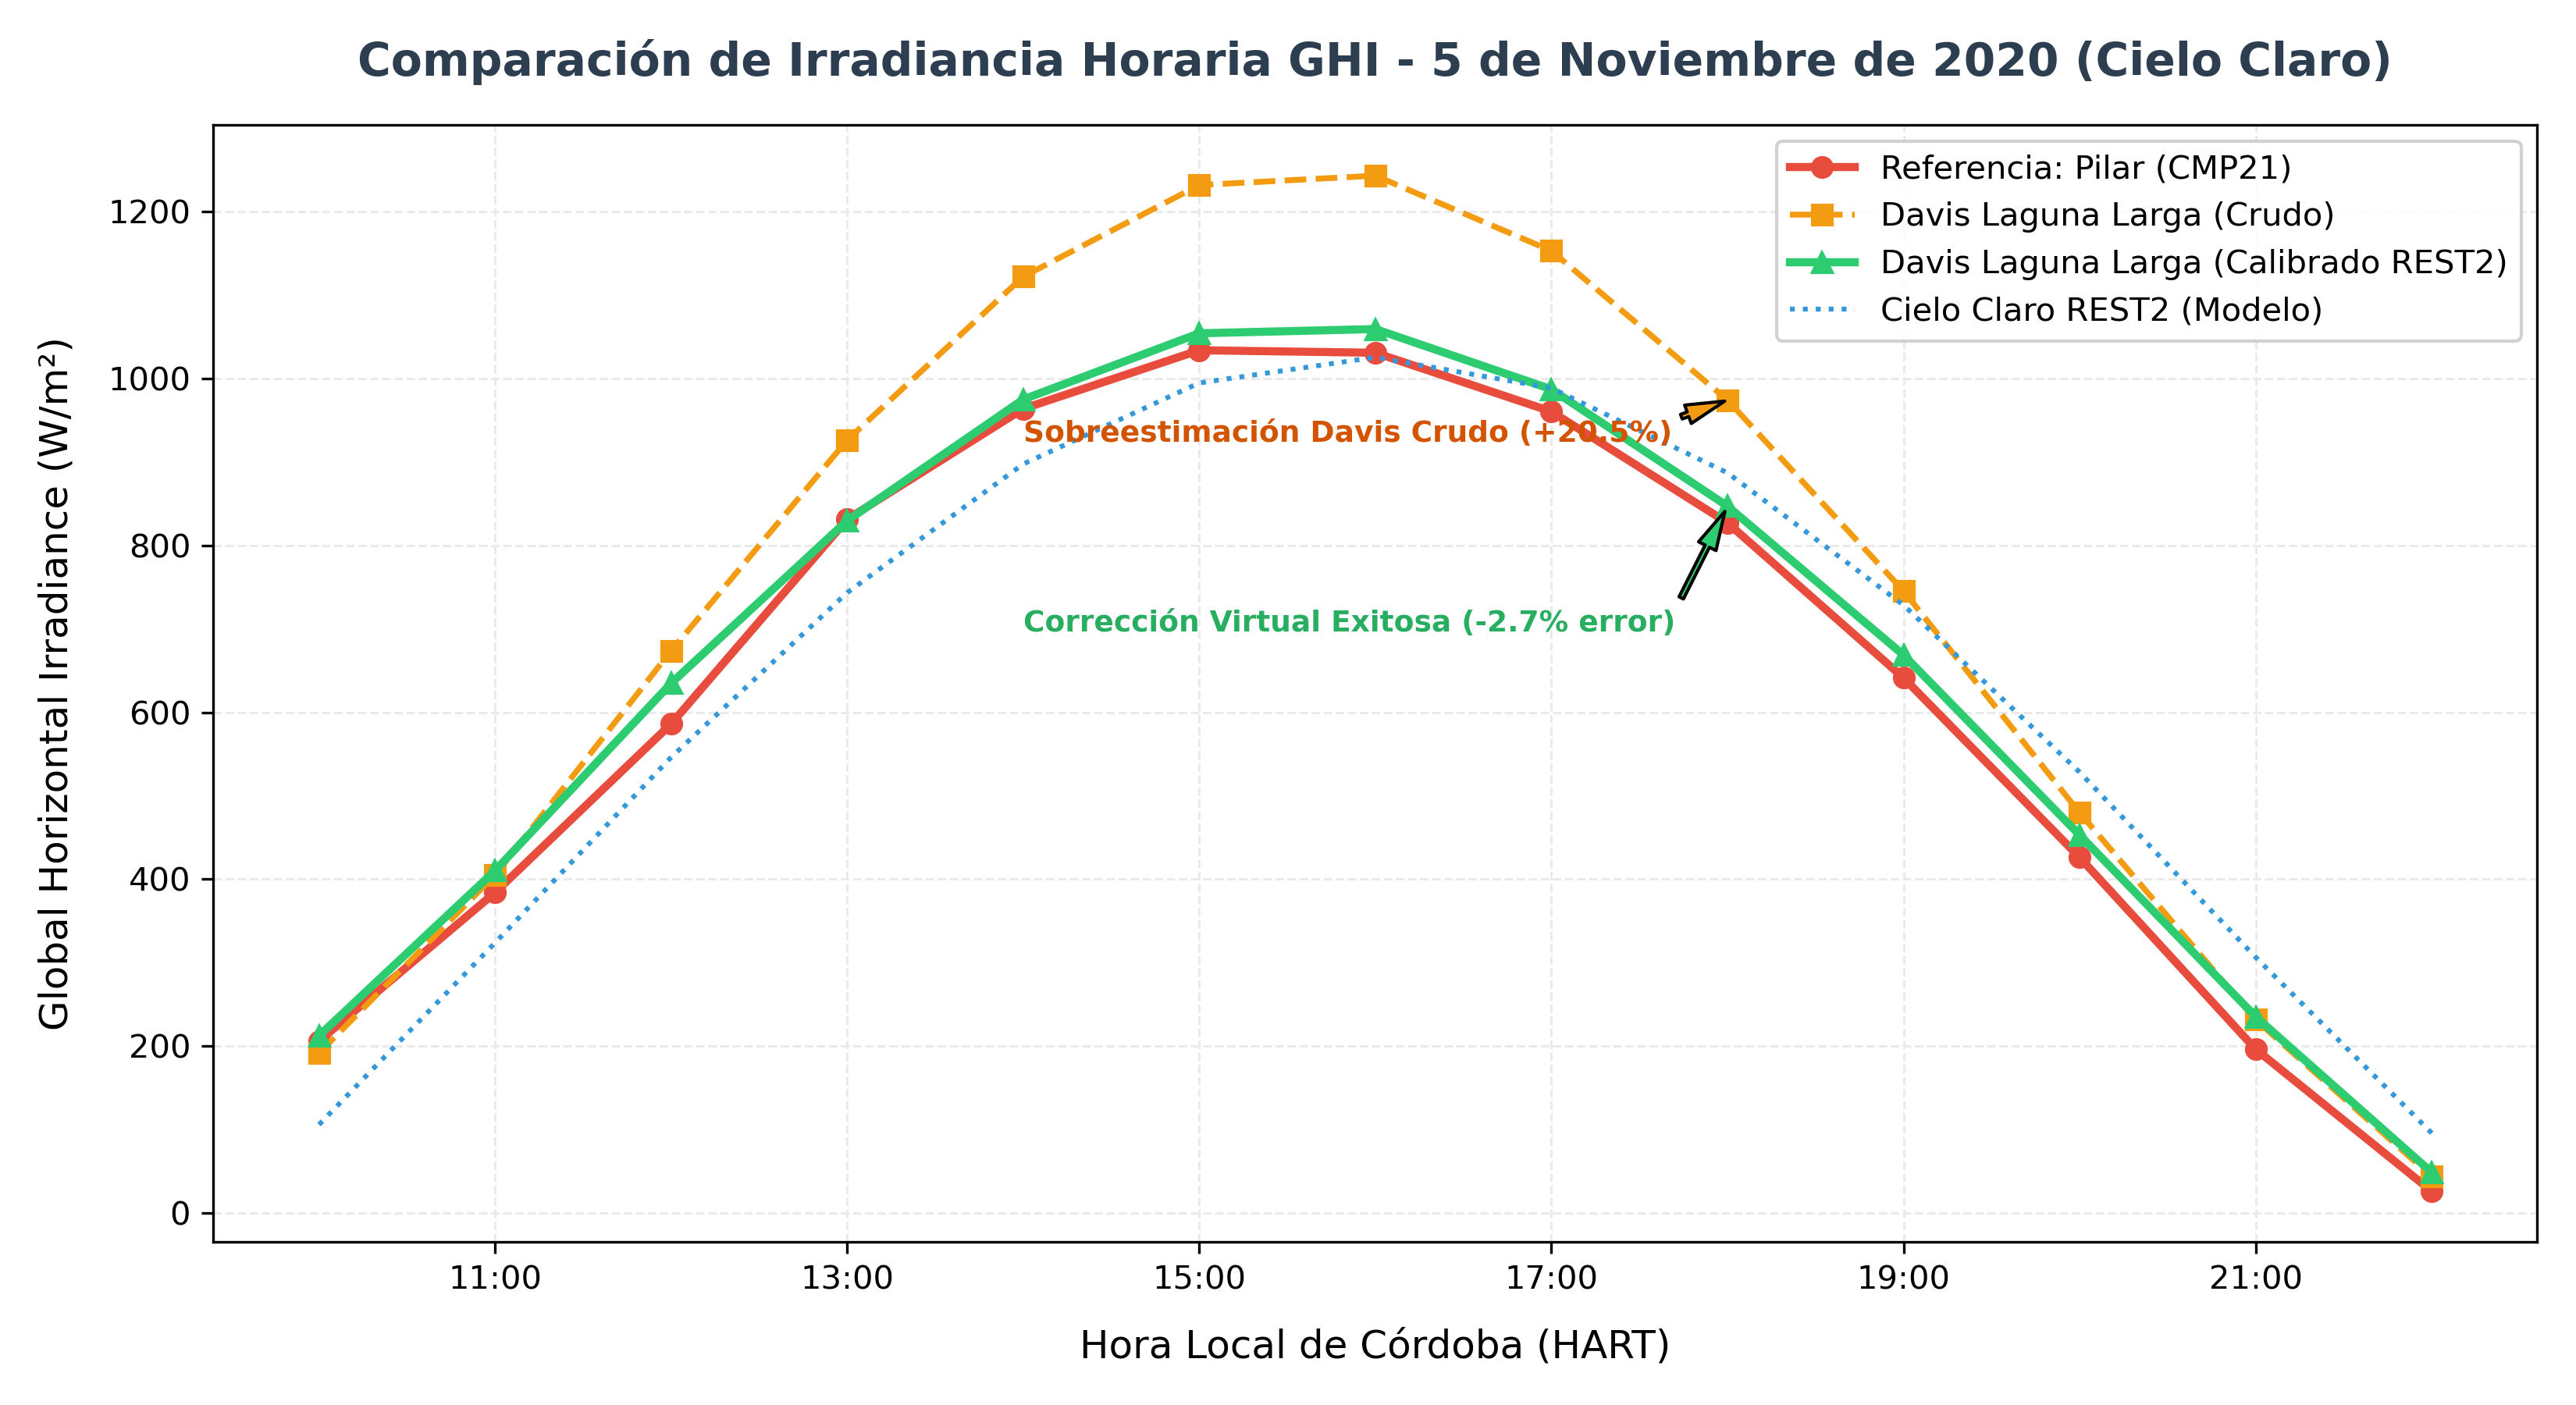
\includegraphics[width=0.95\textwidth]{figuras/figura_3_comparacion_pilar.png}
    \caption{Comparación de GHI entre la estación Davis Laguna Larga, la referencia CMP21 de Pilar y el modelo de cielo claro para el 5 de noviembre de 2020.}
    \label{fig:comparacion_pilar}
\end{figure}

El impacto cuantitativo de la calibración, evaluado sobre el conjunto de horas comparadas, fue el siguiente:

\begin{itemize}
    \item \textbf{Antes de la calibración:} RMSE = $190.65 \text{ W/m}^2$ \;|\; MBE = $+18.75 \text{ W/m}^2$.
    \item \textbf{Después de la calibración:} RMSE = $173.88 \text{ W/m}^2$ \;|\; MBE = $-38.56 \text{ W/m}^2$.
\end{itemize}

La reducción del RMSE, cercana al 9\%, indica una mejora moderada en la consistencia general de la serie calibrada respecto de la referencia CMP21. Sin embargo, el cambio del MBE hacia valores negativos muestra que la calibración introduce una tendencia media a la subestimación en esta comparación agregada. Este resultado no debe interpretarse como una falla directa del procedimiento, sino considerando las limitaciones propias de la validación espacial: aun con una separación relativamente pequeña, una distancia de 12.3 km puede introducir errores de representatividad debido a nubosidad local, aerosoles no capturados adecuadamente por CAMS, diferencias microclimáticas o variabilidad atmosférica submesoescala.

En particular, una nube puede afectar a Pilar y no a Laguna Larga, o viceversa, incrementando el RMSE sin que ello refleje necesariamente un error instrumental. Por este motivo, la validación debe interpretarse principalmente como una prueba de consistencia física y de reducción de sesgos extremos bajo condiciones comparables, más que como una validación punto a punto perfecta.

\textbf{Riesgo de circularidad:} dado que REST2 se utiliza tanto como referencia teórica para la calibración como para evaluar la coherencia física de las series \cite{gueymard_2008_rest2,gueymard_2012_clearsky}, existe un riesgo potencial de circularidad metodológica. La comparación con la estación CMP21 de Pilar, independiente del procedimiento de calibración Davis--REST2, permite reducir este riesgo y aportar una validación empírica externa del comportamiento de la serie corregida.


\newpage


\section{Variabilidad regional de la calibración y regionalización preliminar}

\subsection{Regiones geográficas contrastantes}

Como primera aproximación a la variabilidad espacial de la calibración, se analizaron estaciones representativas de regiones geográficas contrastantes dentro de la Provincia de Córdoba. Este enfoque permite evaluar si las diferencias topográficas, atmosféricas y de emplazamiento modifican la relación entre la señal observada por los sensores Davis y la irradiancia esperada bajo condiciones de cielo claro.

La Figura \ref{fig:curvas_regionales} muestra curvas de calibración polinomial representativas para tres contextos provinciales diferenciados: una zona urbana, una zona serrana y una zona de llanura al sur. Estas curvas evidencian que la corrección no se comporta como un único factor de escala homogéneo para toda la red, sino que presenta variaciones dependientes del ángulo cenital solar y del emplazamiento de la estación.

\begin{figure}[H]
    \centering
    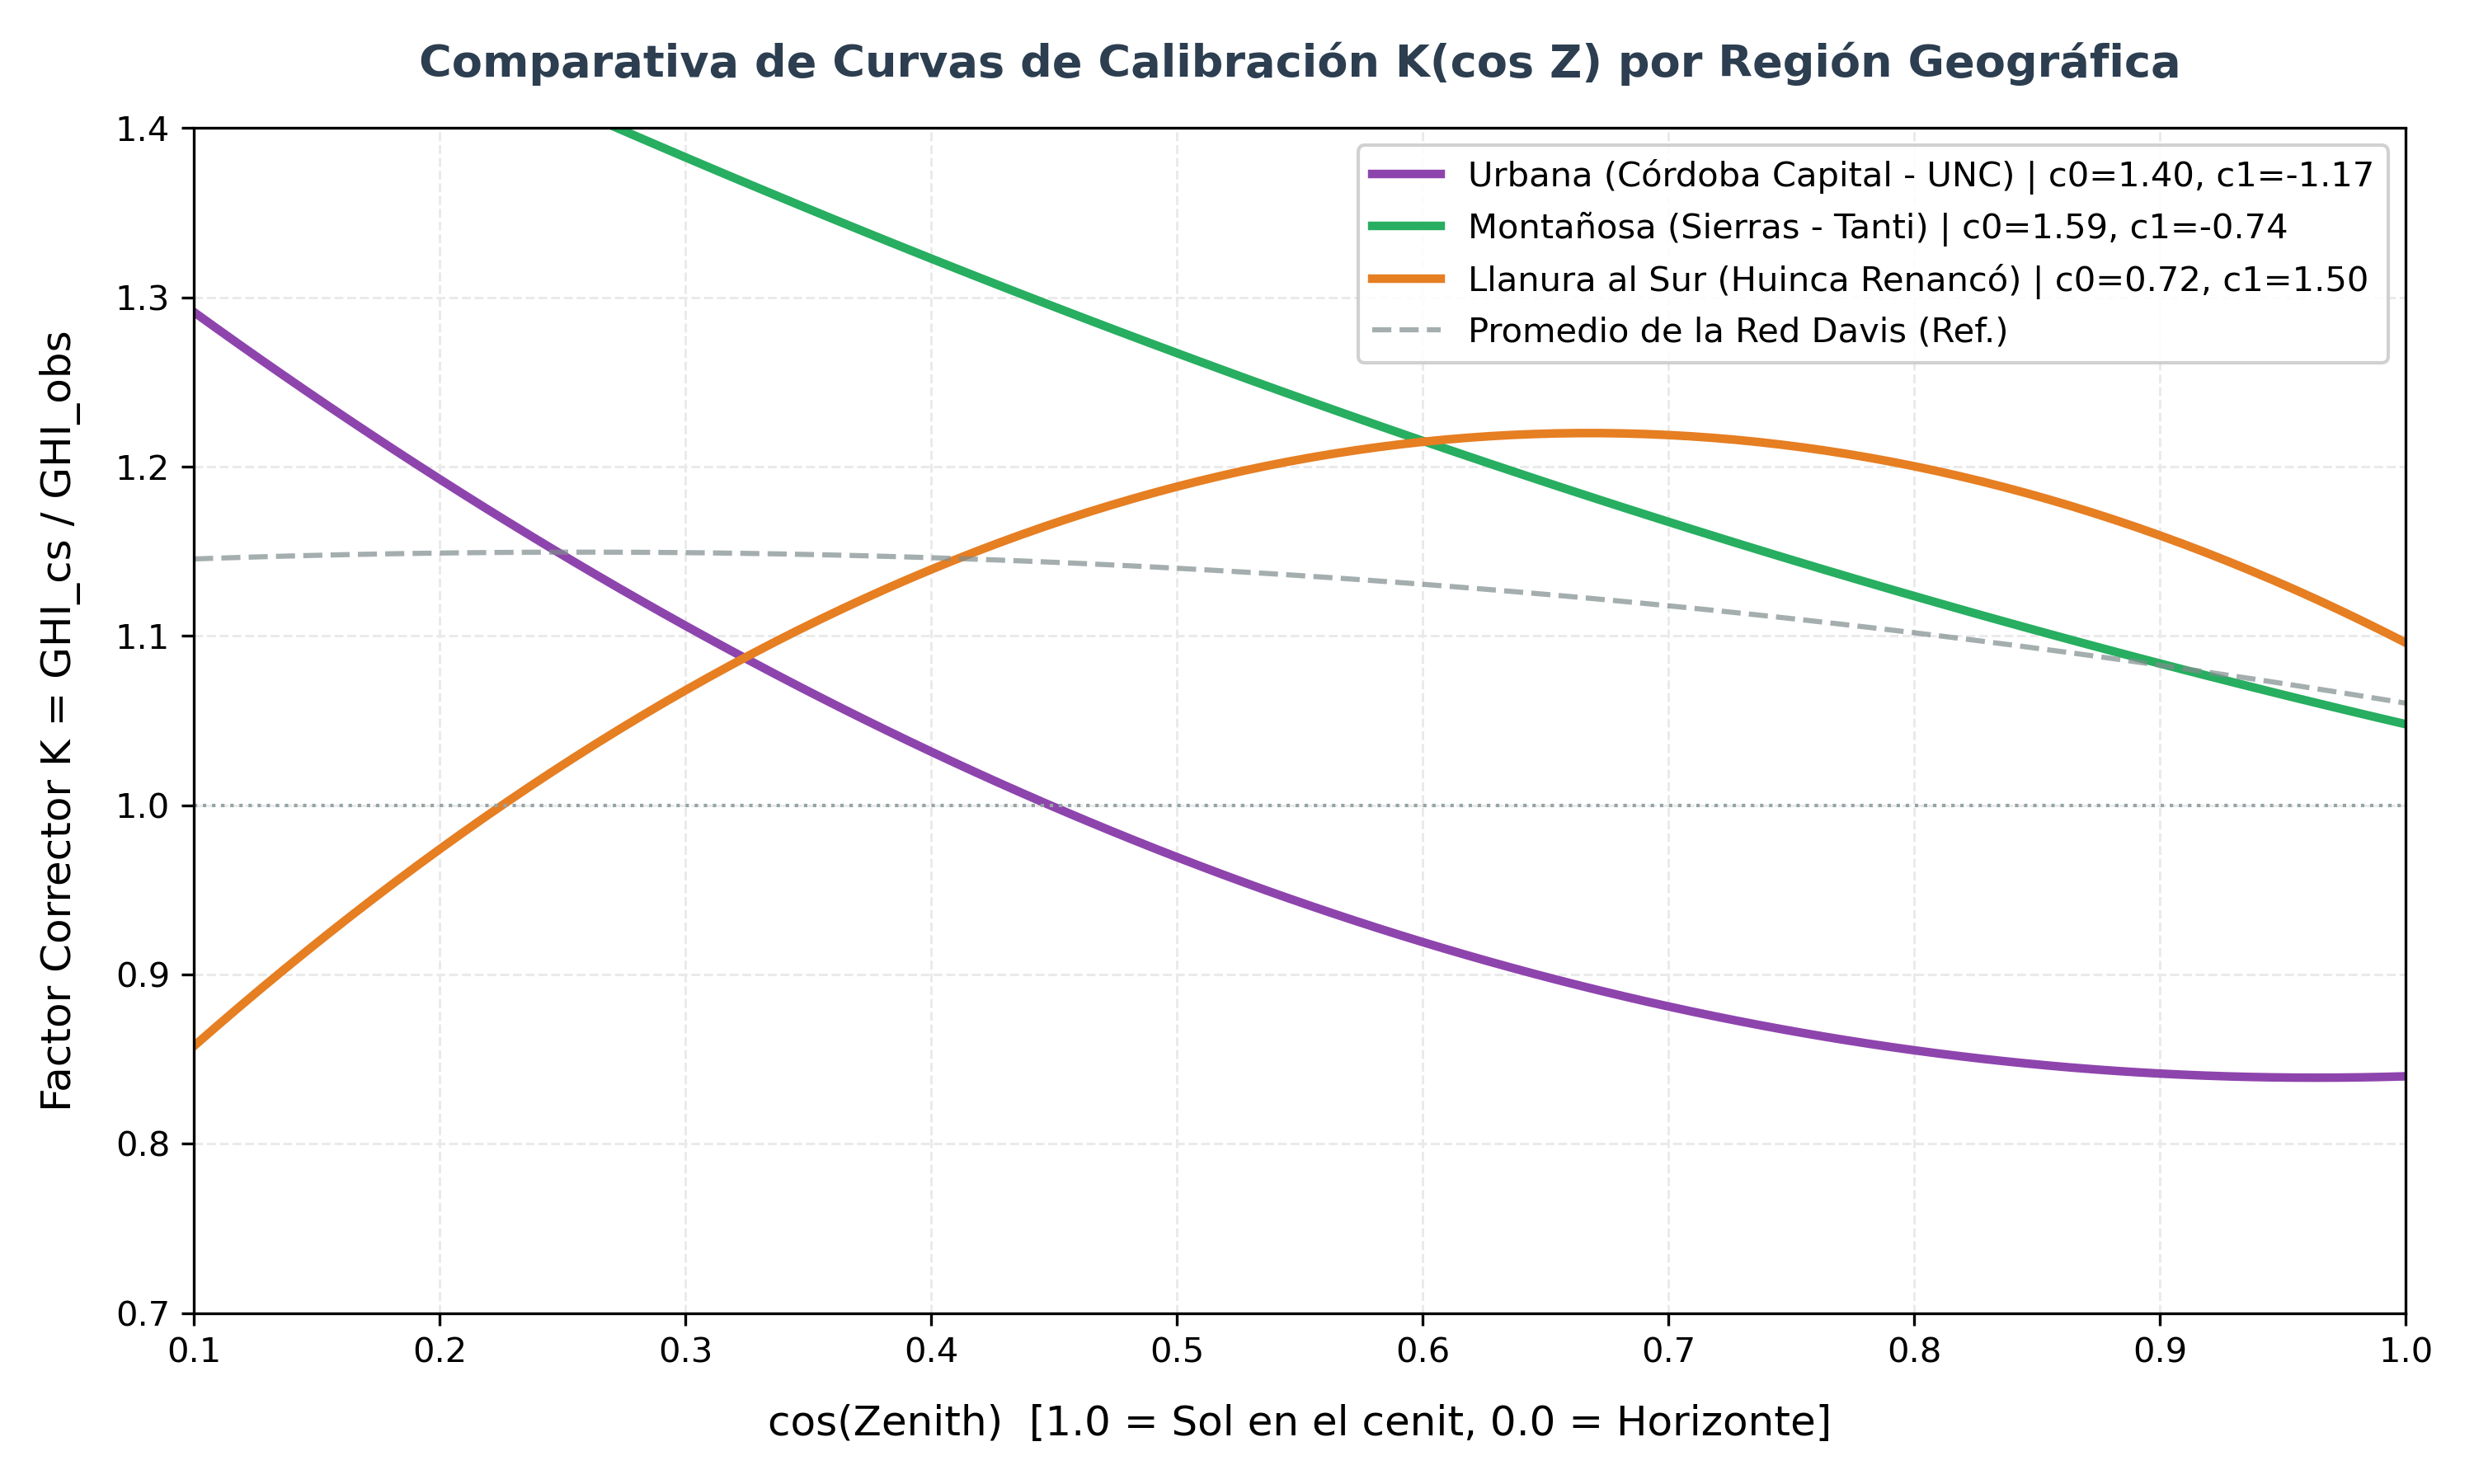
\includegraphics[width=0.75\textwidth]{figuras/figura_8_curvas_regionales.png}
    \caption{Curvas de calibración polinomial representativas para regiones geográficas contrastantes de la Provincia de Córdoba.}
    \label{fig:curvas_regionales}
\end{figure}

La comparación de perfiles horarios en un día despejado refuerza esta interpretación. Como se observa en la Figura \ref{fig:comparacion_regional}, la calibración ajusta de manera diferenciada la señal cruda según el comportamiento local de cada estación, acercando las series corregidas al modelo de cielo claro sin imponer una respuesta uniforme sobre toda la red.

\begin{figure}[H]
    \centering
    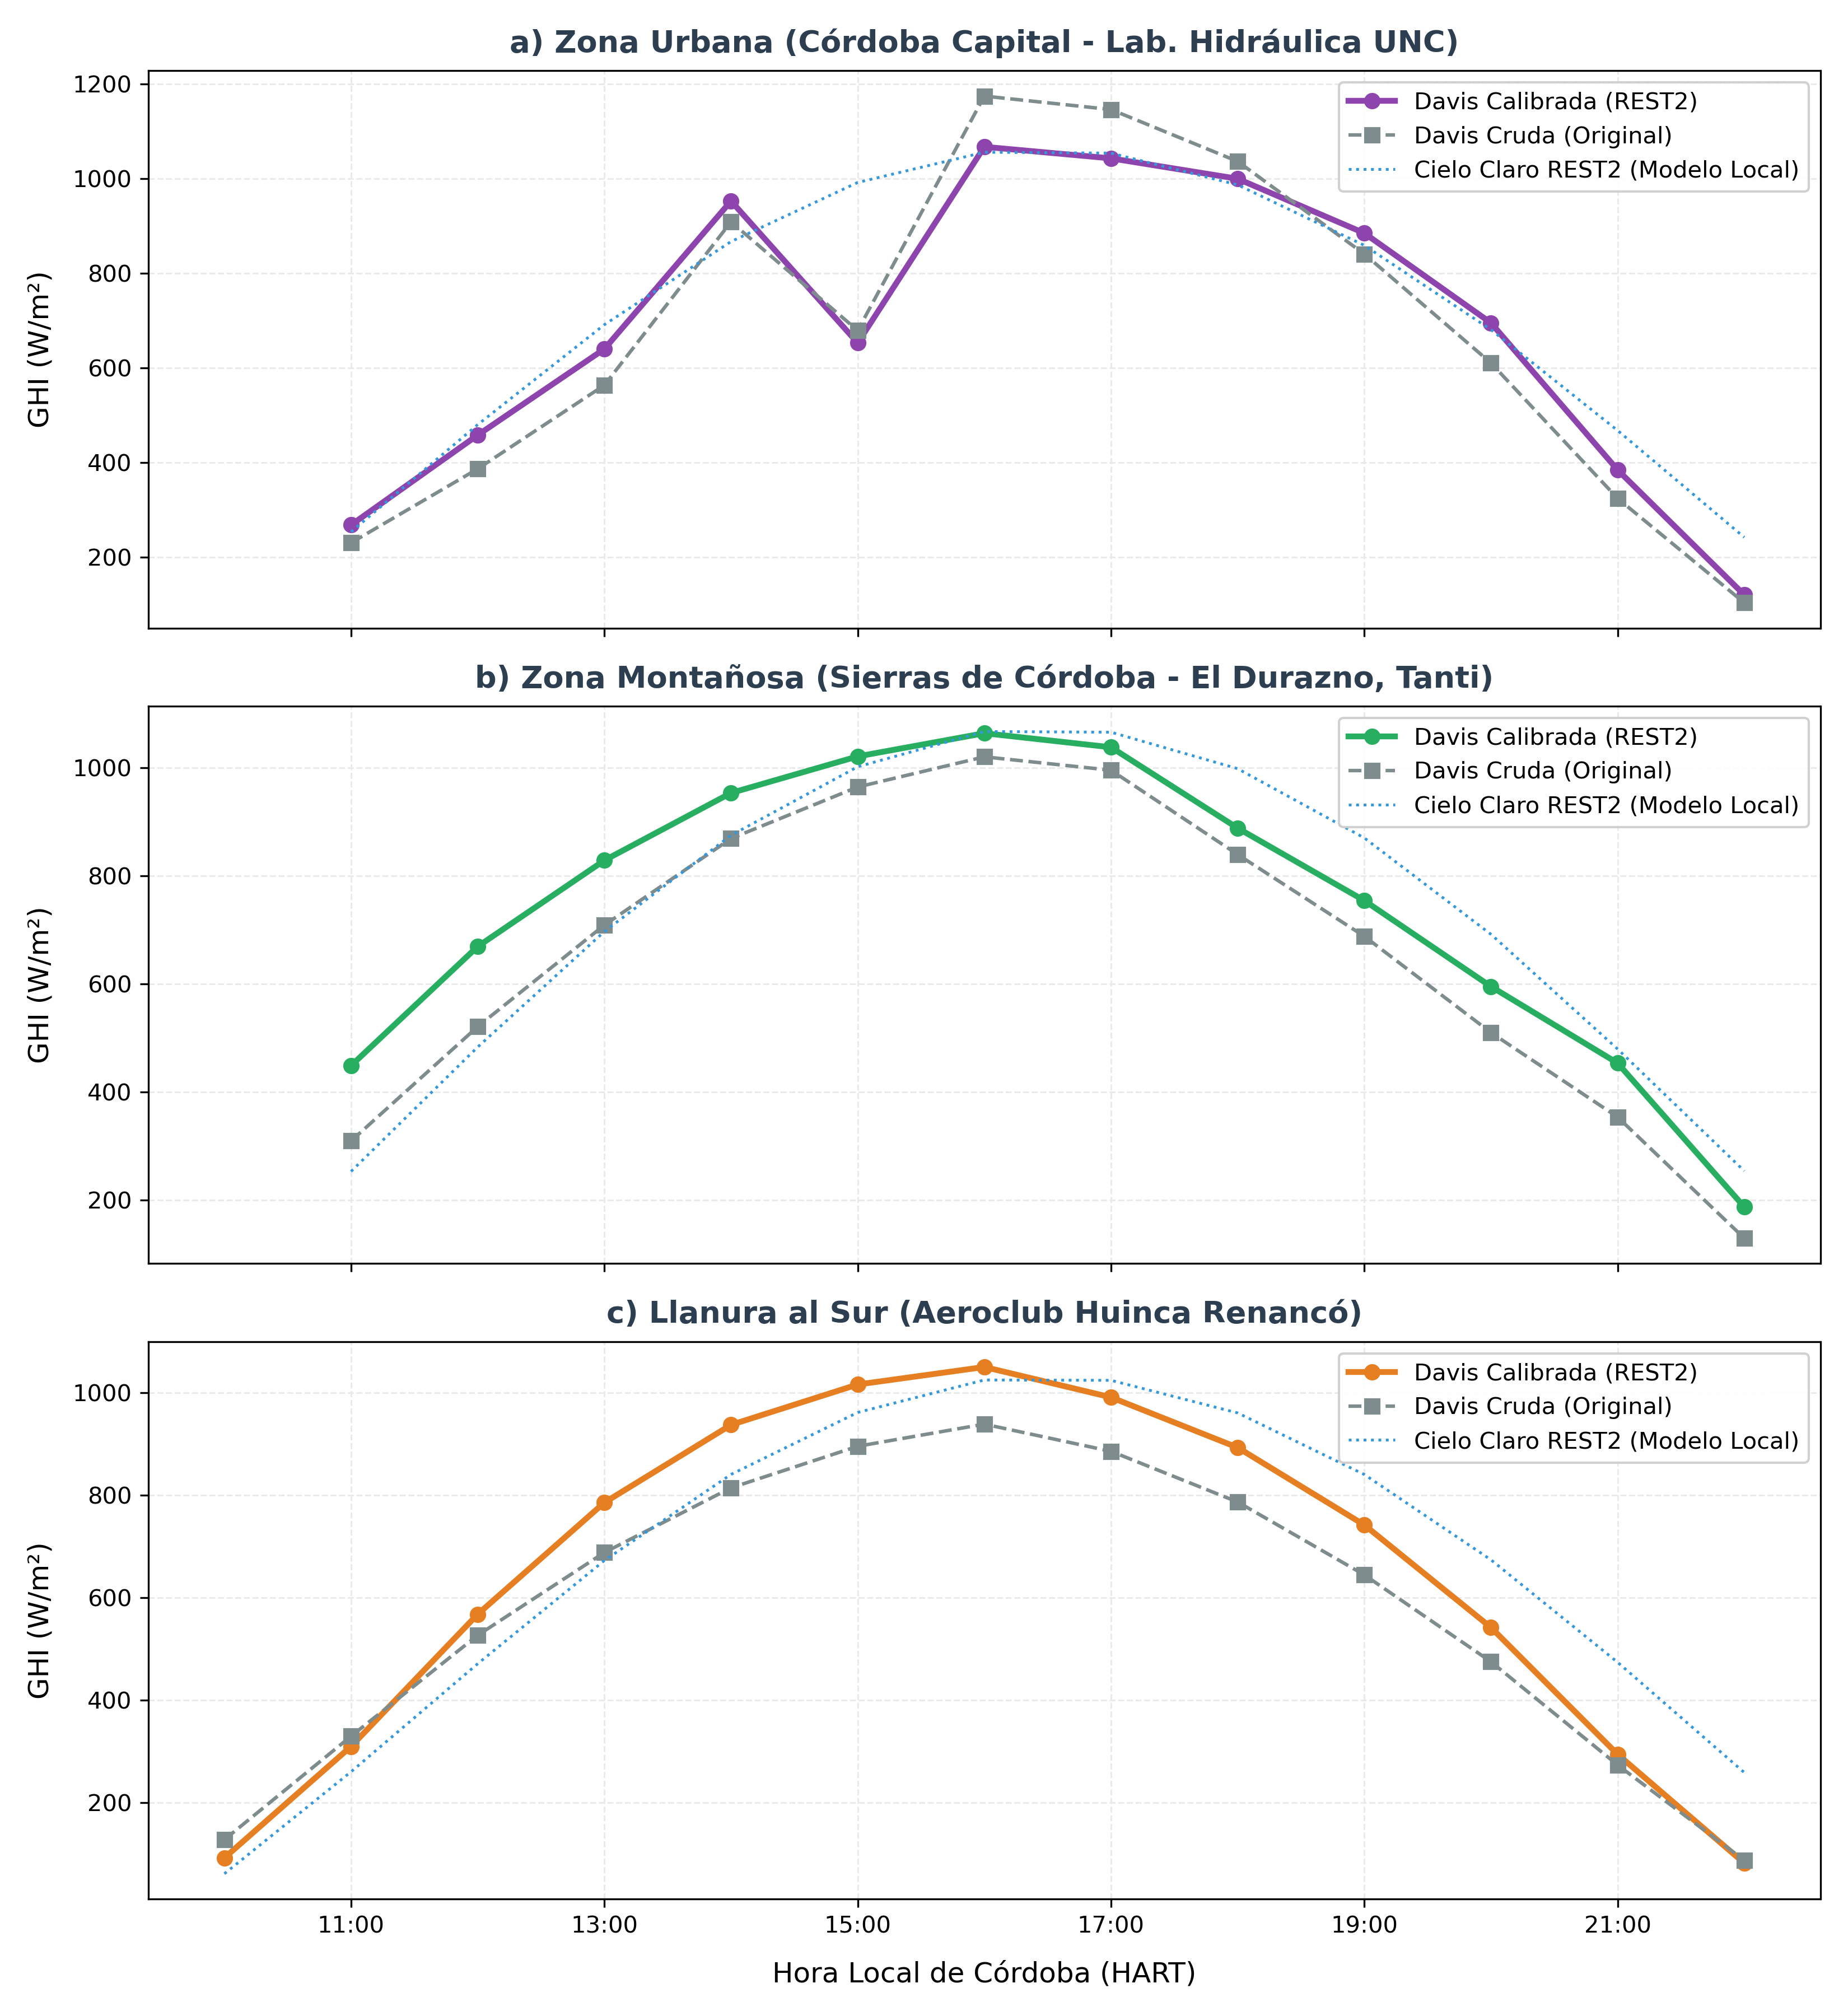
\includegraphics[width=0.9\textwidth]{figuras/figura_9_comparacion_regional.png}
    \caption{Comparación regional de perfiles horarios en un día despejado. Se aprecia la variabilidad de la corrección según el emplazamiento de la estación y su relación con el modelo de cielo claro.}
    \label{fig:comparacion_regional}
\end{figure}


\subsection{Metodología preliminar para la regionalización solar mediante clustering}

De forma complementaria al análisis de estaciones representativas en regiones geográficas contrastantes, se desarrolló una metodología preliminar para evaluar una futura regionalización objetiva del recurso solar provincial. Esta etapa se plantea como insumo para el siguiente informe, en el cual la red terrestre calibrada será integrada con información satelital y atmosférica para avanzar hacia una zonificación espacial más robusta.

El objetivo de esta metodología es identificar agrupamientos de estaciones con comportamiento solar similar, evitando definir regiones únicamente a partir de límites administrativos o criterios visuales. Para ello se propone aplicar un algoritmo de aprendizaje automático no supervisado, \textit{K-Means}, sobre variables físicas y radiométricas derivadas de las estaciones Davis calibradas. Este tipo de enfoque permite agrupar observaciones en función de su similitud multivariada y ha sido utilizado previamente en estudios de regionalización ambiental para la Provincia de Córdoba.

El procedimiento parte de la base horaria de radiación calibrada. En primer lugar, se filtran las horas nocturnas o de muy baja radiación, conservando únicamente los registros con irradiancia teórica de cielo claro mayor a 10 W/m\textsuperscript{2} ($GHI_{cs} > 10$). A partir de estos datos se calcula el índice de claridad:

\begin{equation}
    K_t = \frac{GHI_{\text{obs}}}{GHI_{cs}}
\end{equation}

donde $GHI_{\text{obs}}$ corresponde a la irradiancia observada o calibrada, y $GHI_{cs}$ a la irradiancia estimada por el modelo de cielo claro. Posteriormente, los datos horarios se agregan a escala de estación, obteniendo indicadores medios tales como GHI diurna calibrada, índice de claridad medio y factor de calibración representativo.

Para caracterizar la similitud entre estaciones, estos indicadores radiométricos se combinan con variables geográficas y topográficas. En esta primera implementación se consideran cinco variables principales:

\begin{itemize}
    \item latitud,
    \item longitud,
    \item altitud sobre el nivel del mar,
    \item GHI promedio diurno,
    \item índice de claridad medio ($K_t$).
\end{itemize}

Dado que estas variables poseen unidades y rangos numéricos diferentes, se aplica una estandarización previa mediante \textit{StandardScaler}, transformando cada variable a media cero y varianza unitaria. Este paso evita que variables con mayor amplitud numérica, como la altitud, dominen artificialmente el cálculo de distancias utilizado por el algoritmo.

El número de regiones solares no se impone de manera previa, sino que se evalúa mediante una búsqueda sobre distintas configuraciones de $k$. En particular, se analizan particiones con $k=3$, $k=4$, $k=5$ y $k=6$ clústeres. Para cada configuración se calcula el \textit{Silhouette Score}, una métrica que evalúa la cohesión interna de cada grupo y su separación respecto de los grupos vecinos. Valores más altos indican agrupamientos más compactos y mejor diferenciados.

Los resultados de esta etapa serán utilizados en el siguiente informe para evaluar si existen regiones solares con comportamiento físico diferenciado dentro de la provincia. En caso de obtenerse agrupamientos consistentes, la regionalización podrá emplearse como insumo para el modelado espacial, la calibración satelital y la generación de productos provinciales de irradiancia. De este modo, el análisis de clustering se presenta aquí como una metodología exploratoria en desarrollo, orientada a formalizar una zonificación solar objetiva en etapas posteriores del proyecto.

\section{Conclusiones y transición a la fase satelital}

\subsection{Conclusiones del trabajo terrestre}

La finalización de la calibración de superficie constituye un avance metodológico relevante para la construcción del Atlas Solar Provincial. Los principales resultados de esta etapa pueden resumirse en los siguientes puntos:

\begin{enumerate}
    \item \textbf{Base de datos terrestre unificada y calibrada:} se consolidó un dataset de 166 estaciones con aproximadamente 3.05 millones de horas diurnas útiles, sometidas a control de calidad físico y temporal.

    \item \textbf{Corrección físicamente consistente:} se implementó una calibración dinámica dependiente del ángulo cenital solar, capaz de corregir sesgos espectrales, angulares y de escala característicos de los sensores de silicio de la red Davis.

    \item \textbf{Recuperación de cobertura temporal de largo plazo:} se obtuvieron 39 estaciones con series continuas entre 2019 y 2025, que constituyen un núcleo temporal robusto para caracterizar la variabilidad interanual del recurso solar.

    \item \textbf{Regionalización solar preliminar:} se identificaron 4 regiones solares principales mediante clustering multivariado, proporcionando una primera zonificación física del comportamiento radiativo provincial.
\end{enumerate}

\textbf{Evaluación de incertidumbre:} considerando la incertidumbre asociada a los productos atmosféricos ERA5/CAMS \cite{hersbach_2020_era5,inness_2019_cams}, las limitaciones del modelo de cielo claro \cite{gueymard_2012_clearsky} y la precisión residual observada durante la validación, la incertidumbre horaria esperada del dataset terrestre final de GHI se estima en el rango de $\pm 10-15\%$. Esta estimación debe interpretarse como una incertidumbre operativa de referencia para escalas horarias, susceptible de reducirse al considerar agregaciones diarias, mensuales o climatológicas.

\subsection{Avance del Informe 3}

Los datasets resultantes constituyen la base terrestre calibrada sobre la cual se sustentará la siguiente etapa del proyecto: la calibración satelital y el modelado espacial del recurso solar provincial. En el tercer informe se avanzará en la integración de la red de superficie con información satelital y atmosférica, incluyendo el desarrollo de procedimientos de \textit{downscaling} y la generación de campos espaciales continuos de irradiancia para toda la Provincia de Córdoba.


\newpage

\begin{thebibliography}{99}

\bibitem{long_dutton_2002}
Long, C. N., \& Dutton, E. G. (2002).
\textit{BSRN Global Network recommended QC tests, V2.0}.
BSRN Technical Report.

\bibitem{long_shi_2008}
Long, C. N., \& Shi, Y. (2008).
An automated quality assessment and control algorithm for surface radiation measurements.
\textit{The Open Atmospheric Science Journal}, 2, 23--37.

\bibitem{gueymard_2008_rest2}
Gueymard, C. A. (2008).
REST2: High-performance solar radiation model for cloudless-sky irradiance, illuminance and photosynthetically active radiation.
\textit{Solar Energy}, 82(3), 272--285.
https://doi.org/10.1016/j.solener.2007.04.008

\bibitem{gueymard_2012_clearsky}
Gueymard, C. A. (2012).
Clear-sky irradiance predictions for solar resource mapping and large-scale applications: Improved validation methodology and detailed performance analysis of 18 broadband radiative models.
\textit{Solar Energy}, 86(8), 2145--2169.
https://doi.org/10.1016/j.solener.2011.11.011

\bibitem{hersbach_2020_era5}
Hersbach, H., Bell, B., Berrisford, P., Hirahara, S., Horányi, A., Muñoz-Sabater, J., Nicolas, J., Peubey, C., Radu, R., Schepers, D., Simmons, A., Soci, C., Abdalla, S., Abellan, X., Balsamo, G., Bechtold, P., Biavati, G., Bidlot, J., Bonavita, M., \ldots{} Thépaut, J.-N. (2020).
The ERA5 global reanalysis.
\textit{Quarterly Journal of the Royal Meteorological Society}, 146(730), 1999--2049.
https://doi.org/10.1002/qj.3803

\bibitem{inness_2019_cams}
Inness, A., Ades, M., Agustí-Panareda, A., Barré, J., Benedictow, A., Blechschmidt, A.-M., Dominguez, J. J., Engelen, R., Eskes, H., Flemming, J., Huijnen, V., Jones, L., Kipling, Z., Massart, S., Parrington, M., Peuch, V.-H., Razinger, M., Remy, S., Schulz, M., \& Suttie, M. (2019).
The CAMS reanalysis of atmospheric composition.
\textit{Atmospheric Chemistry and Physics}, 19, 3515--3556.
https://doi.org/10.5194/acp-19-3515-2019

\bibitem{reda_andreas_2004}
Reda, I., \& Andreas, A. (2004).
Solar position algorithm for solar radiation applications.
\textit{Solar Energy}, 76(5), 577--589.
https://doi.org/10.1016/j.solener.2003.12.003

\bibitem{holmgren_2018_pvlib}
Holmgren, W. F., Hansen, C. W., \& Mikofski, M. A. (2018).
pvlib python: a python package for modeling solar energy systems.
\textit{Journal of Open Source Software}, 3(29), 884.
https://doi.org/10.21105/joss.00884

\bibitem{vignola_2017_photodiode}
Vignola, F., Peterson, J., \& Kessler, R. (2017).
Comparison of pyranometers and reference cells on fixed and one-axis tracking surfaces.
In \textit{Proceedings of the ISES Solar World Congress 2017 / IEA SHC International Conference on Solar Heating and Cooling for Buildings and Industry}.
\end{thebibliography}

\end{document}
